\documentclass[
12pt,
fontset=Arno,
lines=36,
chars=80,
bib,
mint,
hyper,
altcolor,
showoverfull,
toclevel=2
]{mbook}

\title{vSMC -- Scalable Monte Carlo}
\author{Yan Zhou}
\date{Release v2.3.0}

\addbibresource{manual.bib}

\NewMinted{c}
\NewMinted{cpp}

\UseAbbr{aes}
\UseAbbr{ais}
\UseAbbr{api}
\UseAbbr{ars}
\UseAbbr{avx}
\UseAbbr{blas}
\UseAbbr{brng}
\UseAbbr{cdf}
\UseAbbr{cpu}
\UseAbbr{crtp}
\UseAbbr{ess}
\UseAbbr{gcc}
\UseAbbr{gnu}
\UseAbbr{gpu}
\UseAbbr{ilp}
\UseAbbr{lapack}
\UseAbbr{llvm}
\UseAbbr{lp}
\UseAbbr{mcmc}
\UseAbbr{mkl}
\UseAbbr{msvc}
\UseAbbr{os}
\UseAbbr{pdf}
\UseAbbr{posix}
\UseAbbr{raii}
\UseAbbr{rdrand}
\UseAbbr{rng}
\UseAbbr{simd}
\UseAbbr{sis}
\UseAbbr{smc}
\UseAbbr{smp}
\UseAbbr{sse}
\UseAbbr{std}
\UseAbbr{stl}
\UseAbbr{tbb}
\UseAbbr{tls}
\UseAbbr{unix}
\UseAbbr{vml}
\UseAbbr{vsl}

\UseAbbr[\aesni][\textsc]{aes-ni}
\UseAbbr[\cnn][\lnfigures\tbfigures\textcase]{C99}
\UseAbbr[\cpp][\textcase]{C++}
\UseAbbr[\cppoo][\lnfigures\tbfigures\textcase]{C++11}
\UseAbbr[\hdf]{hdf5}
\UseAbbr[\io][\textsc]{i/o}
\UseAbbr[\ith][\textsups]{t{}h}
\UseAbbr[\vsmc][]{vSMC}

\UseMathBB{I}
\UseMathCal{N}
\UseMathCal{O}

\def\rmin{r_{\mathrm{min}}}
\def\rmax{r_{\mathrm{max}}}

\def\xobs{X_{\mathrm{obs}}}
\def\xpos{X_{\mathrm{pos}}}
\def\xvel{X_{\mathrm{vel}}}
\def\yobs{Y_{\mathrm{obs}}}
\def\ypos{Y_{\mathrm{pos}}}
\def\yvel{Y_{\mathrm{vel}}}

\def\STATESKIP{\hskip.68cm}

\def\spt{\texttt{SingleParticle<T>}}
\def\wtype{\texttt{weight\_type}}

\newcolumntype{L}{>{\raggedright\arraybackslash}X}
\newcolumntype{R}{>{\raggedleft\arraybackslash}X}

% \includeonly{tex/math}

\begin{document}

\frontmatter
\title{vSMC}
\subtitle{Scalable Monte Carlo}
\author{Yan Zhou}
\date{Release v3.0.0}
\maketitle
\tableofcontents
\listoftables


\mainmatter
\chapter{Introduction}
\label{chap:Introduction}

In this chapter, we introduce the kinds of Monte Carlo algorithms readily
supported by the library and introduce the terminologies used through out this
document.

\section{Resampling}

\section{Markov chain Monte Carlo}

\section{Sequential Monte Carlo}

\chapter{Basic usage}
\label{chap:Basic usage}

\section{Conventions}
\label{sec:Conventions}

All classes that are accessible to users are within the name space \verb|vsmc|.
Class names are in \verb|CamelCase| and function names and class members are in
\verb|small_cases|. In the remaining of this guide, we will omit the
\verb|vsmc::| name space qualifiers. We will use ``function'' for referring to
name space scope functions and ``method'' for class member functions.

\section{Getting and installing the library}
\label{sec:Getting and installing the library}

The library is hosted at
GitHub\footnote{\url{https://github.com/zhouyan/vSMC}}. This is a header only
\cpp template library. To install the library just move the contents of the
\verb|include| directory into a proper place, e.g.,
\verb|/usr/local/include| on Unix-alike systems. This library requires
working \cppoo, \blas and \lapack implementations. Standard C interface headers
for the later two (\verb|cblas.h| and \verb|lapacke.h|) are required. Intel
Threading Building
Blocks\footnote{\url{https://www.threadingbuildingblocks.org}} (\tbb), Intel
Math Kernel Library\footnote{\url{https://software.intel.com/en-us/intel-mkl}}
(\mkl) and \hdf\footnote{\url{http://www.hdfgroup.org}} are optional
third-party libraries. One need to define the configuration macros
\verb|VSMC_HAS_TBB|, \verb|VSMC_HAS_MKL| and \verb|VSMC_HAS_HDF5| to nonzero
values before including any \vsmc headers to make their existence known to the
library, respectively.

\section{Concepts}
\label{sec:Concepts}

The library is structured around a few core concepts. A sampler is responsible
for running an algorithm. It contains a particle system and operations on it. A
particle system is formed by the states $\{X^{(i)}\}_{i=1}^N$ and weights
$\{W^{(i)}\}_{i=1}^N$. This system will also be responsible for resampling. All
user defined operations are to be applied to the whole system. These are
``initialization'' and ``moves'' which are applied before resampling, and
``\mcmc'' moves which are applied after resampling. These operations do not
have to be \mcmc kernels. They can be used for any purpose that suits the
particular algorithm. Most statistical inferences requires calculation of
$\sum_{i=1}^NW^{(i)}\varphi(X^{(i)})$ for some function $\varphi$. This can be
carried out along each sampler iteration by a monitor. Table~\ref{tab:concepts}
lists these concepts and the corresponding types in the library. Each of them
are introduced in detail in the following sections.

\begin{table}
  \begin{tabularx}{\textwidth}{lX}
    \toprule
    Concept & Type \\
    \midrule
    State, $\{X^{(i)}\}_{i=1}^N$            & \verb|T|, user defined   \\
    Weight, $\{W^{(i)}\}_{i=1}^N$           & \verb|Weight|            \\
    Particle, $\{W^{(i)},X^{(i)}\}_{i=1}^N$ & \verb|Particle<T>|       \\
    Single particle, $\{W^{(i)},X^{(i)}\}$  & \verb|SingleParticle<T>| \\
    Sampler        & \verb|Sampler<T>|                                 \\
    Initialization & \verb|Sampler<T>::init_type|, user defined        \\
    Move           & \verb|Sampler<T>::move_type|, user defined        \\
    \mcmc          & \verb|Sampler<T>::mcmc_type|, user defined        \\
    Monitor        & \verb|Monitor<T>|                                 \\
    \bottomrule
  \end{tabularx}
  \caption{Core concepts of the library}
  \label{tab:concepts}
\end{table}

\subsection{State}
\label{sub:State}

The library gives users the maximum flexibility of how the states
$\{X^{(i)}\}_{i=1}^N$ shall be stored and structured. Any class type with a
constructor that takes a single integer value, the number of particles, as its
argument, and a method named \verb|copy| is acceptable. For example,
\begin{cppcode*}{texcomments}
  class T
  {
      public:
      T(std::size_t N);

      template <typename IntType>
      void copy(std::size_t N, IntType *index)
      {
          for (std::size_t i = 0; i != N; ++i) {
              // Let $a_i =$ index[i], set $X^{(i)} = X^{(a_i)}$
          }
      }
  };
\end{cppcode*}
How the state values are actually stored and accessed are entirely up to the
user. The method \verb|copy| is necessary since the library assumes no
knowledge of the internal structure of the state. And thus it cannot perform
the last step of a resampling algorithm, which makes copies of particles with
larger weights and eliminate those with smaller weights.

For most applications, the values can be stored within an $N$ by $d$ matrix,
where $d$ is the dimension of the state. The library provides a convenient
class template for this situation,
\begin{cppcode}
  template <MatrixLayout Layout, std::size_t Dim, typename T>
  class StateMatrix;
\end{cppcode}
where \verb|Layout| is either \verb|RowMajor| or \verb|ColMajor|, which
specifies the matrix storage layout; \verb|Dim| is a non-negative integer
value. If \verb|Dim| is zero, then the dimension may be changed at runtime. If
it is positive, then the dimension is fixed and cannot be changed at runtime.
The last template parameter \verb|T| is the \cpp type of state space. The
following constructs an object of this class,
\begin{cppcode}
  StateMatrix<ColMajor, Dynamic, double> s(N);
\end{cppcode}
where \verb|Dynamic| is just an enumerator with value zero. We can specify the
dimension at runtime through the method \verb|s.resize_dim(d)|. Note that, if
the template parameter \verb|Dim| is positive, then this call results in a
runtime error.

To access $X_{ij}$, the value of the state of the $i$\ith particle at the
$j$\ith coordinate, one can use the method \verb|s.state(i,j)|. The method
\verb|s.data()| returns a pointer to the beginning of the matrix. If
\verb|Layout| is \verb|RowMajor|, then the method \verb|s.row_data(i)| returns
a pointer to the beginning of the $i$\ith row. If \verb|Layout| is
\verb|ColMajor|, then the method \verb|s.col_data(j)| returns a pointer to the
beginning of the $j$\ith column. These methods help interfacing with numerical
libraries, such as \blas.

Apart from \verb|resize_dim|, the matrix can also be resized by the sample size
or both. \verb|s.resize(N, dim)| is the most general form. Let $n$ be the
minimum of the original and new sample sizes, and $d$ be the minimum of the
original and new dimensions. The $n$ by $d$ matrix at the upper left corner of
the original matrix is preserved. If the matrix is enlarged in either
direction, new values will be inserted and default initialized. For more
sophisticated resizing, use the \verb|copy| method, which will create a new set
of states according to the index vector.

\subsection{Weight}
\label{sub:Weight}

The vector of weights $\{W^{(i)}\}_{i=1}^N$ is abstracted in the library by the
\verb|Weight| class. The following constructs an object of this class,
\begin{cppcode}
  Weight w(N);
\end{cppcode}
There are a few methods for accessing the weights,
\begin{cppcode*}{texcomments}
  w.ess();          // Get {\normalfont\textsc{ess}}
  w.set_equal();    // Set $W^{(i)} = 1/N$
\end{cppcode*}
The weights can be manipulated, given a vector of length $N$, say $v$,
\begin{cppcode*}{texcomments}
  w.set(v);         // Set $W^{(i)} \propto v^{(i)}$
  w.mul(v);         // Set $W^{(i)} \propto W^{(i)} v^{(i)}$
  w.set_log(v);     // Set $\log W^{(i)} = v^{(i)} + \text{const.}$
  w.add_log(v);     // Set $\log W^{(i)} = \log W^{(i)} + v^{(i)} + \text{const.}$
\end{cppcode*}
The method \verb|w.data()| returns a pointer to the normalized weights. It is
important to note that the weights are always normalized and all mutable
methods only allow access to $\{W^{(i)}\}_{i=1}^N$ as a whole.

\subsection{Particle}
\label{sub:Particle}

A particle system is composed of both the state values, which is of user
defined type, say \verb|T|, and the weights. The following constructs an object
of class \verb|Particle<T>|,
\begin{cppcode}
  Particle<T> particle(N);
\end{cppcode}
The method \verb|particle.value()| returns the type \verb|T| object. The object
containing the weights is returned by \verb|particle.weight()|. Its type is
\verb|Particle<T>::weight_type|, whose definition depends on the type \verb|T|.
See section~\ref{sec:Customizing member types} for more details. If the user
does not do something special as shown in that section, then the default type
is the \verb|Weight|. They are constructed with the same integer value $N$ when
the above constructor is invoked.

As a Monte Carlo algorithm, random number generators (\rng) will be used
frequently. The user is free to use whatever \rng mechanism as they see fit.
However, one common issue encountered in practice is how to maintain
independence of the \rng streams between function calls. For example, consider
below a function that manipulates some state values,
\begin{cppcode}
  void function(double &x)
  {
      std::mt19937 rng;
      std::normal_distribution<double> rnorm(0, 1);
      x = rnorm(rng);
  }
\end{cppcode}
Every call of this function will give \verb|x| exactly the same value. This is
hardly what the user intended. One might consider an global \rng or one as
class member data. For example,
\begin{cppcode}
  std::mt19937 rng;
  void function(double &x)
  {
      std::normal_distribution<double> rnorm(0, 1);
      x = rnorm(rng);
  }
\end{cppcode}
This will work fine as long as the function is never called by two threads at
the same time. However, \smc algorithms are natural candidates to
parallelization. Therefore, the user will need to either lock the \rng, which
degenerates the performance, or construct different \rng{}s for different
threads. The later, though ensures thread-safety, has other issues. For
example, consider
\begin{cppcode*}{texcomments}
  std::mt19937 rng1(s1); // For thread $i_1$ with seed $s_1$
  std::mt19937 rng2(s2); // For thread $i_2$ with seed $s_2$
\end{cppcode*}
where the seeds $s_1 \ne s_2$. It is difficult to ensure that the two streams
generated by the two \rng{}s are independent. Common practice for parallel \rng
is to use sub-streams or leap-frog algorithms. Without going into any further
details, it is sufficient to say that this is perhaps not a problem that most
users bother to solve.

The library provides a simple solution to this issue. The method
\verb|particle.rng(i)| returns a reference to an \rng that conforms to the
\cppoo uniform \rng concept. It can be called from different threads at the
same time, for example,
\begin{cppcode*}{texcomments}
  auto &rng1 = particle.rng(i1); // Called from thread $i_1$
  auto &rng2 = particle.rng(i2); // Called from thread $i_2$
\end{cppcode*}
If $i_1 \ne i_2$, then the subsequent use of the two \rng{}s are guaranteed to
be thread-safe. In addition, they will produce independent streams. If \tbb is
available to the library, then it is also thread-safe even if $i_1 = i_2$. One
can write functions that process each particle, for example,
\begin{cppcode*}{texcomments}
  void function(std::size_t i)
  {
      auto &rng = particle.rng(i);
      // Process the particle i using rng
  }
\end{cppcode*}
And if later this function is called from a parallelized environment, it is
still thread-safe and produce desired statistical results. The details of the
\rng system are documented later in chapter~\ref{chap:Random number generating}.

\subsubsection{Resize the particle system}

The particle system can be resized. However, the library does not provide a
simple \verb|resize| method that works the same way as \verb|std::vector|, etc.
When a particle system is resized, it is often done through some deterministic
or stochastic algorithms. At least some particles will be preserved and
possibly replicated. The \verb|Particle<T>| class has a few methods for
resizing using different user input to determine the particles to be preserved.
All these methods use \verb|T::copy| to resize the state vector. Therefore, if
any of them need to be used, then the call \verb|copy(N, index)| need to be
able to handle the situation where its first argument has a value other than
its original size. After the resizing, the weights are set to be equal except
\verb|reszie_by_range| below. All methods are discussed in the following
paragraphs.

\paragraph{Resize by selecting according to a user supplied index vector}

\begin{cppcode}
  template <typename InputIter>
  void resize_by_index(size_type N, InputIter index);
\end{cppcode}
The input iterator \verb|index| shall point to a length $N$ vector. Each
element is the parent index of the corresponding new particle. The new system
is formed by $\bar{X}^{(i)} = X^{(a_i)}$ where $a_i$ is the $i$\ith element of
the index vector.

\paragraph{Resize by selecting according to a user supplied mask vector}

\begin{cppcode}
  template <typename InputIter>
  void resize_by_mask(size_type N, InputIter mask);
\end{cppcode}
The input iterator \verb|mask| shall point to a length $n$ vector, where $n$ is
the original sample size. For each element, when converted to \verb|bool|, if
it is \verb|true|, then the corresponding particle is preserved. Otherwise it
is discarded. If there are more than $N$ particles to be preserved, then only
the first $N$ particles are copied into the new system. If there are less than
$N$ particles to be preserved, then the vector of these particles are copied
repeatedly until there are enough particles to fill the new system.

\paragraph{Resize by resampling}

\begin{cppcode}
  template <typename ResampleType>
  void resize_by_resample(size_type N, ResampleType &&op);
\end{cppcode}
The details of the resampling operation function object is discussed in
chapter~\ref{chap:Resampling}. For now, it is sufficient to say that, to use
any of the builtin schemes, one can call the method like the following,
\begin{cppcode}
  particle.resize_by_resample(N, ResampleMultinomial());
\end{cppcode}
This method produce a new particle system by using the specified resampling
algorithm. Note that, this is different from resampling a particle system in
that, all operations are local. That is, if the particle is in a distributed
system, only local weights are used, and re-normalized.

\paragraph{Resize by uniformly selecting from all particles}

\begin{cppcode}
  void resize_by_uniform(size_type N);
\end{cppcode}
This is equivalent to,
\begin{cppcode}
  particle.weight().set_equal();
  particle.resize_by_resample(N, ResampleMultinomial());
\end{cppcode}

\paragraph{Resize by selecting a range of particles}

\begin{cppcode}
  void resize_by_range(size_type N, size_type first, size_type last);
\end{cppcode}
This is the most destructive resizing method. Let $n = \text{last} -
\text{first}$. If $n < N$,the particles in the range $[\text{first},
\text{last})$ are copied repeatedly until there are enough particles to fill
the new system. Otherwise only the first $N$ particles are copied. If
\verb|last| is omitted, then it is set to \verb|size()|. If \verb|first| is
also omitted, then it is set to zero. Use this method only when the statistical
properties of the new system is irrelevant. If one want to avoid the copying
altogether, it might be more efficient to simply create a new system with
the desired size. This method is a no-op if $N$ is the same as the original
size.

\subsection{Single particle}
\label{sub:Single particle}

It is often easier to define a function $f(X^{(i)})$ than
$f(X^{(1)},\dots,X^{(N)})$. However, \verb|Particle<T>| only provides access to
$\{X^{(i)}\}_{i=1}^N$ as a whole through \verb|particle.value()|. To allow
direct access to $X^{(i)}$, the library uses a class template
\verb|SingeParticle<T>|. An object of this class is constructed from the index
$i$ of the particle, and a pointer to the particle system it belongs to,
\begin{cppcode}
  SingleParticle<T> sp(i, &particle);
\end{cppcode}
or more conveniently,
\begin{cppcode}
  auto sp = particle.sp(i);
\end{cppcode}
In its most basic form, it has the following methods,
\begin{cppcode}
  sp.id();       // Get the value i that sp was constructed with
  sp.particle(); // Get a reference to the Particle<T> object sp belongs to
  sp.rng();      // => sp.particle().rng(sp.id());
\end{cppcode}
If \verb|T| is a derived class of \verb|StateMatrix|, then it has two
additional methods,
\begin{cppcode}
  sp.dim();    // => sp.particle().value().dim();
  sp.state(j); // => sp.particle().value().state(sp.id(), j);
\end{cppcode}
It is clear now that the interface of \verb|SingleParticle<T>| depends on the
type \verb|T|. Later in section~\ref{sec:Extending SP} we will show how to
insert additional methods into this class.

A \verb|SingleParticle<T>| object is similar to an iterator. In fact, it
supports almost all of the operations of a random access iterator with two
exceptions. First dereferencing a \verb|SingleParticle<T>| object returns
itself. The support of \verb|operator*| allows the range-based for loop to be
applied on a \verb|Particle<T>| object, for example,
\begin{cppcode}
  for (auto sp : particle) {
      // sp is of type SingleParticle<T>
  }
\end{cppcode}
The above loop does make some sense. However trying to dereferencing a
\verb|SingleParticle<T>| object in other contexts does not make much sense.
Recall that it is an \emph{index}, not a \emph{pointer}. The library does not
require the user defined type \verb|T| to provide access to individual values,
and thus it cannot dereference a \verb|SingleParticle<T>| object to obtain such
a value. Similarly, the expression \verb|sp[n]| returns \verb|sp + n|, another
\verb|SingleParticle<T>| object. For the same reason, \verb|operator->| is not
supported at all.

\subsection{Sampler}
\label{sub:Sampler}

A sampler can be constructed in a few ways,
\begin{cppcode}
  Sampler<T> sampler(N);
\end{cppcode}
constructs a sampler that is never resampled, while
\begin{cppcode}
  Sampler<T> sampler(N, Multinomial);
\end{cppcode}
constructs a sampler that is resampled every iteration, using the multinomial
algorithm. Other resampling schemes are also implemented, see
chapter~\ref{chap:Resampling}. Last, one can also construct a sampler that is
only resampled when $\ess < \alpha N$, where $\alpha\in[0, 1]$, by the
following,
\begin{cppcode}
  Sampler<T> sampler(N, Multinomial, alpha);
\end{cppcode}
If $\alpha > 1$, then it has the same effect as the first constructor, since
$\ess \le N$. If $\alpha < 0$, then it has the same effect as the second
constructor, since $\ess > 0$.

In summary, if one does not tell the constructor which resampling scheme to
use, then it is assumed one does not want to do resampling. If one specify the
resampling scheme without a threshold for \ess, then it is assumed it need to
be done at every step.

The method \verb|sampler.particle()| returns a reference to the particle
system. A sampler can be initialized by user defined object that is convertible
to the following type,
\begin{cppcode}
  using init_type = std::function<std::size_t(Particle<T> &, void *)>;
\end{cppcode}
For example,
\begin{cppcode}
  auto init = [](Particle<T> &particle, void *param) {
      // Process initialization parameter
      // Initialize the particle system
  };
\end{cppcode}
is a \cppoo lambda expression that can be used for this purpose. One can add it
to a sampler by calling \verb|sampler.init(init)|. Upon calling
\verb|sampler.initialize(param)|, the user defined function \verb|init| will be
called and the argument \verb|param| will be passed to it.

Similarly, after initialization, at each iteration, the particle system can be
manipulated by user defined callable objects that is convertible to the
following types,
\begin{cppcode}
  using move_type = std::function<std::size_t(std::size_t, Particle<T> &)>;
  using mcmc_type = std::function<std::size_t(std::size_t, Particle<T> &)>;
\end{cppcode}
Multiple moves can be added to a sampler. The call
\verb|sampler.move(move, append)| adds a \verb|move_type| object to the
sampler, where \verb|append| is a boolean value. If it is \verb|false|, it will
clear any moves that were added before. If it is \verb|true|, then \verb|move|
is appended to the end of an existing sequence of moves. Each move will be
called one by one upon calling \verb|sampler.iterate()|. A similar sequence of
\mcmc moves can also be added to a sampler. The call \verb|sampler.iterate()|
will call user defined moves first, then perform the possible resampling, and
then the sequence of \mcmc moves.

Note that the possible resampling will also be performed after the user defined
initialization function is called by \verb|sampler.initialize(param)|. And
after that, the sequence of \mcmc moves will be called. If it desired not to
perform mutations during initialization, then following can be used,
\begin{cppcode}
  sampler.init(init).initialize(param);
  sampler.move(move, false).mcmc(mcmc, false).iterate(n);
\end{cppcode}
The above code also demonstrates that most methods of \verb|Sampler<T>| return
a reference to the sampler itself and thus method calls can be chained. In
addition, method \verb|sampler.iterate(n)| accepts an optional argument that
specifies the number of iterations. It is a shortcut for
\begin{cppcode}
  for (std::size_t i = 0; i != n; ++i)
      sampler.iterate();
\end{cppcode}

\subsection{Monitor}
\label{sub:Monitor}

Inferences using a \smc algorithm usually require the calculation of the
quantity $\sum_{i=1}^NW^{(i)}\varphi(X^{(i)})$ at each iteration for some
function $\varphi$. One can define callable object that is convertible to the
following type,
\begin{cppcode}
  using eval_type =
      std::function<void(std::size_t, std::size_t, Particle<T> &, double *);
\end{cppcode}
For example,
\begin{cppcode*}{texcomments}
  void eval(std::size_t iter, std::size_t d, Particle<T> &particle, double *r)
  {
      for (std::size_t i = 0; i != particle.size(); ++i, r += dim) {
          auto sp = particle.sp(i);
          r[0] = /* $\varphi_1(X^{(i)})$ */;
          // ...
          r[d - 1] = /* $\varphi_d(X^{(i)})$ */;
      }
  }
\end{cppcode*}
The argument \verb|d| is the dimension of the vector function $\varphi$. The
output is an $N$ by $d$ matrix in row major layout, with each row corresponding
to the value of $\varphi(X^{(i)})$. Then one can add this function to a sampler
by calling,
\begin{cppcode}
  sampler.monitor("name", d, eval);
\end{cppcode}
where the first argument is the name for the monitor, the second its dimension,
and the third the evaluation function. At each iteration, after all the
initialization, possible resampling, moves and \mcmc moves are done, the
sampler will calculate $\sum_{i=1}^NW^{(i)}\varphi(X^{(i)})$. This method has
two optional arguments. First is a boolean value \verb|record_only|. If it is
\verb|true|, it is assumed that no summation is needed. For example,
\begin{cppcode*}{texcomments}
  void eval(std::size_t iter, std::size_t d, Particle<T> &particle, double *r)
  {
      r[0] = /* $\varphi_1(\{X^{(i)}\}_{i=1}^N)$ */;
      // ...
      r[d - 1] = /* $\varphi_d(\{X^{(i)}\}_{i=1}^N)$ */;
  }
\end{cppcode*}
In this case, the monitor acts merely as a storage facility. The second
optional argument is \verb|stage| which specifies at which point the monitoring
shall happen. It can be \verb|MonitorMove|, which specifies that the monitoring
happens right after the moves and before resampling. It can also be
\verb|MonitorResample|, which specifies that the monitoring happens right after
the resampling and before the \mcmc moves. Last, the default is
\verb|MonitorMCMC|, which specifies that the monitoring happens after
everything.

The output of a sampler, together with the records of any monitors it has can
be output in plain text forms through a \cpp output stream. For example,
\begin{cppcode}
  std::cout << sampler;
\end{cppcode}
We will see how this works later with a concrete particle filter example. If
the \hdf library is available, it is also possible to write such output to \hdf
format, for example,
\begin{cppcode}
  hdf5store(sampler, file_name, data_name);
\end{cppcode}
Details can be found in section~\ref{sec:Store objects in HDF5 format}.

\section{A simple particle filter}
\label{sec:A simple particle filter}

\subsection{Model and algorithm}
\label{sub:Model and algorithm}

This is an example used in \textcite{Johansen:2009wd}. Through this example, we
will show how to re-implement a simple particle filter in \vsmc. It shall walk
one through the basic features of the library introduced above.

The state space model, known as the almost constant velocity model in the
tracking literature, provides a simple scenario. The state vector $X_t$
contains the position and velocity of an object moving in a plane. That is,
$X_t = (\xpos^t, \ypos^t, \xvel^t, \yvel^t)^T$. Imperfect observations $Y_t =
(\xobs^t, \yobs^t)^T$ of the positions are possible at each time instance. The
state and observation equations are linear with additive noises,
\begin{align*}
  X_t &= AX_{t-1} + V_t \\
  Y_t &= BX_t + \alpha W_t
\end{align*}
where
\begin{equation*}
  A = \begin{pmatrix}
    1 & \Delta & 0 & 0 \\
    0 & 1 & 0 & 0 \\
    0 & 0 & 1 & 0 \\
    0 & 0 & 0 & 1
  \end{pmatrix} \qquad
  B = \begin{pmatrix}
    1 & 0 & 0 & 0 \\
    0 & 1 & 0 & 0 \\
  \end{pmatrix} \qquad
  \alpha = 0.1
\end{equation*}
and we assume that the elements of the noise vector $V_t$ are independent
Gaussian with variance $0.02$ and $0.001$ for position and velocity,
respectively. The observation noise, $W_t$ comprises independent, identically
distributed $t$-distributed random variables with degree of freedom $\nu = 10$.
The prior at time $0$ corresponds to an axis-aligned Gaussian with variance $4$
for the position coordinates and $1$ for the velocity coordinates. The particle
filter algorithm is shown in algorithm~\ref{alg:pf}.

\begin{algorithm}[t]
  \begin{algorithmic}
    \hrule\vskip1ex
    \STATE \emph{Initialization}
    \STATE\STATESKIP Set $t\leftarrow0$.
    \STATE\STATESKIP Sample
    $\xpos^{(0,i)},\ypos^{(0,i)}\sim\calN(0,4)$ and
    $\xvel^{(0,i)},\yvel^{(0,i)}\sim\calN(0,1)$.
    \STATE\STATESKIP Weight $W_0^{(i)} \propto \exp{\ell(X_0^{(i)}|Y_0)}$ where
    $\ell$ is the likelihood function.

    \STATE \emph{Iteration}
    \STATE\STATESKIP Set $t\leftarrow t + 1$.
    \STATE\STATESKIP Sample
    \begin{align*}
      \xpos^{(t,i)}&\sim\calN(\xpos^{(t-1,i)} + \Delta\xvel^{(t-1,i)}, 0.02) &
      \xvel^{(t,i)}&\sim\calN(\xvel^{(t-1,i)}, 0.001) \\
      \ypos^{(t,i)}&\sim\calN(\ypos^{(t-1,i)} + \Delta\yvel^{(t-1,i)}, 0.02) &
      \yvel^{(t,i)}&\sim\calN(\yvel^{(t-1,i)}, 0.001)
    \end{align*}
    \STATE\STATESKIP Weight $W_t^{(i)} \propto
    W_{t-1}^{(i)}\exp{\ell(X_t^{(i)}|Y_t)}$.

    \STATE \emph{Repeat the \emph{Iteration} step until all data are processed}.
    \vskip1ex\hrule
  \end{algorithmic}
  \caption{Particle filter algorithm for the almost constant velocity model.}
  \label{alg:pf}
\end{algorithm}

\subsection{Implementations}
\label{sub:Implementations}

The complete program is shown in appendix~\appref{app:sub:Sequential
  implementation}. In this section we show the outline of the implementation.

\subsubsection{The main program}

\begin{cppcode}
    Sampler<PFState> sampler(N, Multinomial, 0.5);
    sampler.init(PFInit()).move(PFMove(), false).monitor("pos", 2, PFEval());
    sampler.initialize(const_cast<char *>("pf.data")).iterate(n - 1);

    std::ofstream output("pf.out");
    output << sampler;
    output.close();
\end{cppcode}
\verb|Sampler<PFState>| object is constructed first. Then the initialization
\verb|PFInit|, move \verb|PFMove| and a monitor \verb|PFEval| that records
$\xpos^t$ and $\ypos^t$ are added to the sampler. The monitor is named
\verb|"pos"|. Then it is initialized with the name of the data file
\verb|"pf.data"|, and iterated $n - 1$ times, where $n$ is the number of data
points. At last, the output is written into a text file \verb|"pf.out"|. Below
is a short R\footnote{\url{http://r-project.org}} script that can be used to
process the output
\begin{rcode}
  library(ggplot2)

  pf <- read.table("pf.out", header = TRUE)
  sink("pf.rout")
  print(pf[1:5,])
  sink()

  obs <- read.table("pf.data", header = FALSE)
  dat <- data.frame(
  X = c(pf[["pos.0"]], obs[,1]),
  Y = c(pf[["pos.1"]], obs[,2]))
  dat[["Source"]] <- rep(c("Estimate", "Observation"), each = dim(obs)[1])
  plt <- qplot(x = X, y = Y, data = dat, geom = "path")
  plt <- plt + aes(group = Source, color = Source, linetype = Source)
  plt <- plt + theme_bw() + theme(legend.position = "top")
  pdf("pf.pdf")
  print(plt)
  dev.off()
\end{rcode}
The \verb|print| statement shows the first five lines of the output,
\begin{textcode}
    Size Resampled Accept.0      ESS    pos.0   pos.1
  1 1000         1        0   2.9204 -1.21951 3.16397
  2 1000         1        0 313.6830 -1.15602 3.22770
  3 1000         1        0  33.0421 -1.26451 3.04031
  4 1000         1        0  80.1088 -1.45922 3.37625
  5 1000         1        0 382.8820 -1.47299 3.49230
\end{textcode}
The column \verb|Size| shows the sample size at each iteration. The column
\verb|Resampled| shows nonzero values if resampling were performed and zero
otherwise. For each moves and \mcmc steps, an acceptance count will be
recorded. In this particular example, it is irrelevant. Next the column
\verb|ESS| shows the value of \ess. The last two columns show the importance
sampling estimates of the positions recorded by the monitor named \verb|"pos"|.
The graphical representation of the output is shown in figure~\ref{fig:pf}.

\begin{figure}
  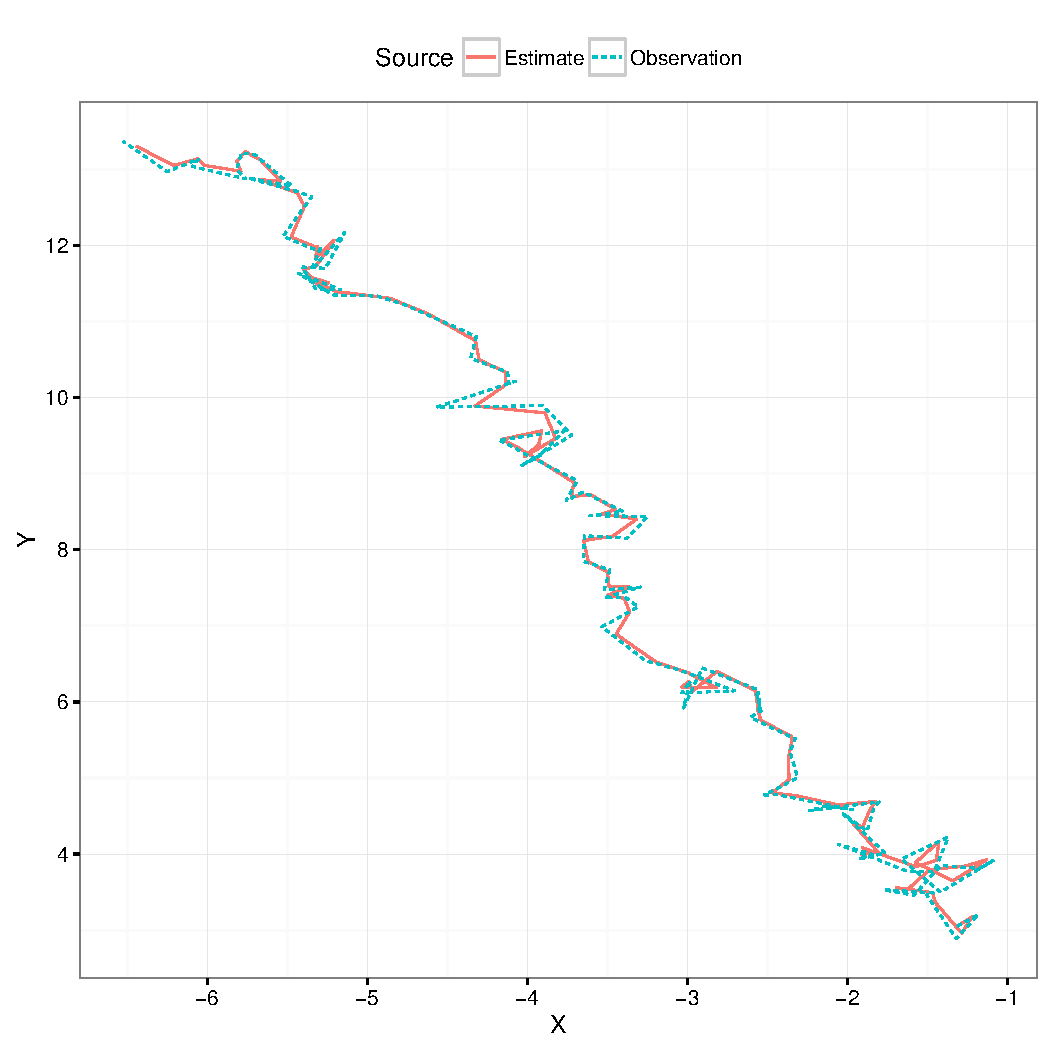
\includegraphics[width=\linewidth]{cpp/pf}
  \caption{A simple particle filter}
  \label{fig:pf}
\end{figure}

Before diving into the details of the implementation of \verb|PFState|, etc.,
we will first define a few constant and types. The state space is of dimension
$4$. And it is natural to use a \verb|StateMatrix| as the base class of
\verb|PFState|,
\begin{cppcode}
  using PFStateBase = StateMatrix<RowMajor, 4, double>;
\end{cppcode}
The numbers of particles and data points are also defined as constants in this
simple example,
\begin{cppcode}
  static constexpr std::size_t N = 1000; // Number of particles
  static constexpr std::size_t n = 100;  // Number of data points
\end{cppcode}
Last, we define the following constants as the indices of each state component.
\begin{cppcode}
  static constexpr std::size_t PosX = 0;
  static constexpr std::size_t PosY = 1;
  static constexpr std::size_t VelX = 2;
  static constexpr std::size_t VelY = 3;
\end{cppcode}

\subsubsection{State: \texttt{PFState}}

As noted earlier, \verb|StateMatrix| will be used as the base class of
\verb|PFState|. Since the data will be shared by all particles, we also store
the data within this class. And methods will be provided to read the data from
an external file, and compute the log-likelihood $\ell(X^{(i)})$, which
accesses the data. Below the declaration of the class \verb|PFState| is shown,
\begin{cppcode*}{texcomments}
  class PFState : public PFStateBase
  {
      public:
      using PFStateBase::PFStateBase;

      // Return $\ell(X_t^{(i)}|Y_t)$
      double log_likelihood(std::size_t t, size_type i) const;

      // Read data from an external file
      void read_data(const char *param);

      private:
      Vector<double> obs_x_;
      Vector<double> obs_y_;
  };
\end{cppcode*}

\subsubsection{Initialization: \texttt{PFInit}}

The initialization step is implemented as below,
\begin{cppcode}
  class PFInit
  {
      public:
      std::size_t operator()(Particle<PFState> &particle, void *param)
      {
          eval_param(particle, param);
          eval_pre(particle);
          std::size_t acc = 0;
          for (auto sp : particle)
              acc += eval_sp(sp);
          eval_post(particle);

          return acc;
      }

      void eval_param(Particle<PFState> &particle, void *param)
      {
          particle.value().read_data(static_cast<const char *>(param));
      }

      void eval_pre(Particle<PFState> &particle)
      {
          weight_.resize(particle.size());
      }

      std::size_t eval_sp(SingleParticle<PFState> sp)
      {
          NormalDistribution<double> norm_pos(0, 2);
          NormalDistribution<double> norm_vel(0, 1);
          sp.state(PosX) = norm_pos(sp.rng());
          sp.state(PosY) = norm_pos(sp.rng());
          sp.state(VelX) = norm_vel(sp.rng());
          sp.state(VelY) = norm_vel(sp.rng());
          w_[sp.id()] = sp.particle().value().log_likelihood(0, sp.id());

          return 0;
      }

      void eval_post(Particle<PFState> &particle)
      {
          particle.weight().set_log(weight_.data());
      }

      private:
      Vector<double> weight_;
  };
\end{cppcode}
An object of this class is convertible to \verb|Sampler<PFState>::init_type|.
In the main method, \verb|operator()|, \verb|eval_param| is called first to
initialize the data. Then \verb|eval_pre| is called to allocated any resource
this class need before calling any \verb|eval_sp|. In this case, it allocate
the vector \verb|w_| for storing weights computed later. Next, the main loop
initializes each state component with the respective Gaussian distribution,
computes the log-likelihood and store them in the vector allocated in the last
step. This is done by calling the \verb|eval_sp| method. After all particles
have been initialized, we set the weights of the system in \verb|eval_post|.
Later in section~\ref{sec:Symmetric multiprocessing} it will become clear why
we structured the implementation this way.

\subsubsection{Move: \texttt{PFMove}}

The move step is similar to the initialization. We show the declaration here,
\begin{cppcode}
  class PFMove
  {
      public:
      std::size_t operator()(std::size_t t, Particle<PFState> &particle);
      void eval_pre(std::size_t t, Particle<PFState> &particle);
      std::size_t eval_sp(std::size_t t, SingleParticle<PFState> sp);
      void eval_post(std::size_t t, Particle<PFState> &particle);

      private:
      Vector<double> w_;
  };
\end{cppcode}

\subsubsection{Monitor: \texttt{PFEval}}

Last we define \verb|PFEval|, which simply copies the values of the positions.
\begin{cppcode}
  class PFEval
  {
      public:
      void operator()(std::size_t t, std::size_t dim,
          Particle<PFState> &particle, double *r)
      {
          eval_pre(t, particle);
          for (std::size_t i = 0; i != particle.size(); ++i, r += dim)
              eval_sp(t, dim, particle.sp(i), r);
          eval_post(t, particle);
      }

      void eval_pre(std::size_t t, Particle<PFState> &particle) {}

      void eval_sp(std::size_t t, std::size_t dim,
          SingleParticle<PFState> sp, double *r)
      {
          r[0] = sp.state(PosX);
          r[1] = sp.state(PosY);
      }

      void eval_post(std::size_t t, Particle<PFState> &particle) {}
  };
\end{cppcode}

\section{Symmetric multiprocessing}
\label{sec:Symmetric multiprocessing}

The above example is implemented in a sequential fashion. However, the loops
inside \verb|PFInit|, \verb|PFMove| and \verb|PFEval| clearly can be
parallelized. The library provides basic support of multicore parallelization
through its \smp module. Two widely used backends, OpenMP and \tbb are
available. Here we demonstrate how to use the \tbb backend. First we will
declare the implementation classes as derived classes,
\begin{cppcode}
  class PFInit : public InitializationTBB<PFState>;
  class PFMove : public MoveTBB<PFState>;
  class PFEval : public MonitorEvalTBB<PFState>;
\end{cppcode}
And remove \verb|operator()| from their implementations. After these changes,
the implementation will be parallelized using \tbb. The complete program can be
found in section The complete program is shown in
appendix~\appref{app:sub:Parallelized implementation using TBB}.

It works as if \verb|InitializationTBB<PFState>| has an implementation of
\verb|operator()| as we did before, except it is parallelized. Now it is clear
that, method such as \verb|eval_pre| and \verb|eval_post| are called before and
after the main loop. Method \verb|eval_sp| is called within the loop and it
need to be thread-safe if called with different arguments. This is the main
reason we constructed the \verb|NormalDistribution| objects within
\verb|eval_sp| instead of as member data, even though they are constructed in
exactly the same way for each particle. This is because
\verb|NormalDistribution::operator()| is a mutable method and thus not
thread-safe. If any of these member functions does not do anything, then it
does not have to be defined in the derived class.

Apart from the three base classes we have shown here, there are also
\verb|InitializationOMP|, etc., for using the OpenMP backend. And
\verb|InitializationSEQ|, etc., for implementation without parallelization. The
later works in exactly the same way as our implementation in the last section.
It is often easier to debug a single-threaded program than a parallelized one.
And thus one may develop the algorithm with the sequential backend and obtain
optimal performance latter by only changing the name of a few base class names.
This can usually be done automatically through a build system.

\subsection{Performance consideration}
\label{sec:Performance consideration}

The base classes dispatch calls to \verb|eval_pre|, \verb|eval_sp|, etc.,
through the virtual function mechanism. The performance impact is minimal for
\verb|eval_pre| and \verb|eval_post|, since they are called only once in each
iteration and we expect the computational cost will be dominated by
\verb|eval_sp| in most cases. However, the dynamic dispatch can cause
considerable performance degenerating if the cost of a single call to
\verb|eval_sp| is small while the number of particles is large. Modern
optimizing compilers can usually devirtualize the method calls in trivial
situations. However, it is not always possible. In this situation, the library
will need a little help from the user to make compile-time dispatch. For each
implementation class, we will declare it in the following way,
\begin{cppcode}
  class PFInit : public InitializationTBB<PFState, PFInit>;
  class PFMove : public MoveTBB<PFState, PFMove>;
  class PFEval : public MonitorEvalTBB<PFState, PFEval>;
\end{cppcode}
The second template argument of the base class need to be exactly the same as
the derived class. For interested users, this is called Curiously Recurring
Template
Pattern\footnote{\url{https://en.wikipedia.org/wiki/Curiously_recurring_template_pattern}}
(\crtp). This usage of the library's base classes also provides other
flexibility. The methods \verb|eval_pre| etc., can be either \verb|const| or
mutable. They can also be \verb|static|.

\chapter{Advanced usage}
\label{chap:Advanced usage}

\section{Cloning objects}
\label{sec:Cloning objects}

The \verb|Sampler<T>| and \verb|Particle<T>| objects have copy constructors,
assignment operators, move constructors, and move assignment operators that
behave exactly the way as \cpp programmers would expect. However, these
behaviors are not always desired. For example, in \textcite{stpf} a stable
particle filter in high-dimensions was developed. Without going into the
details, the algorithm consists of a particle system where each particle is
itself a particle filter. And thus when resampling the global system, the
\verb|Sampler<T>| object will be copied, together with all of its sub-objects.
This include the \rng system within the \verb|Particle<T>| object. Even if the
user does not use this \rng system for random number generating within user
defined operations, one of these \rng will be used for resampling by the
\verb|Particle<T>| object. Direct copying the \verb|Sampler<T>| object will
lead to multiple local filters start generating exactly the same random numbers
in the next iteration. This is an undesired side effect. In this situation, one
can clone the sampler with the following method,
\begin{Verbatim}
  auto new_sampler = sampler.clone(new_rng);
\end{Verbatim}
where \verb|new_rng| is a boolean value. If it is \verb|true|, then an exact
copy of \verb|sampler| will be returned, except it will have the \rng system
re-seeded. If it is \verb|false|, then the above assignemnt behaves exactly the
same as
\begin{Verbatim}
  auto new_sampler = sampler;
\end{Verbatim}
Alternatively, the contents of an existing \verb|Sampler<T>| object can be
replaced from another one by the following method,
\begin{Verbatim}
  sampler.clone(other_sampler, retain_rng);
\end{Verbatim}
where \verb|retain_rng| is a boolean value. If it is \verb|true|, then the \rng
system of \verb|other_sampler| is not copied and the original is retained. If
it is \verb|false|, then the above call behaves exactly the same as
\begin{Verbatim}
  sampler = other_sampler;
\end{Verbatim}
The above method also supports move semantics. Similar \verb|clone| methods
exist for the \verb|Particle<T>| class.

\section{Customizing member types}
\label{sec:Customizing member types}

The \verb|Particle<T>| class has a few member types that can be replaced by the
user. If the class \verb|T| has the corresponding types, then the member type
of \verb|Particle<T>| will be replaced. For example, given the following
declarations inside class \verb|T|,
\begin{Verbatim}
  class T
  {
      public:
      using size_type = int;
      using weight_type = /* User defined type */;
      using rng_set_type = RNGSetTBB<AES256_4x32>;
  };
\end{Verbatim}
The corresponding \verb|Particle<T>::size_type|, etc., will have their defaults
replaced with the above types.

\subsection{Replacing \protect\wtype}
\label{sub:Replacing wtype}

The class for managing the weights needs to provide the following methods,
\begin{Verbatim}
  w.ess();           // Get $\text{\normalfont\textsc{ess}}$
  w.set_equal();     // Set $W^{(i)} = 1/N$
  w.resample_size(); // Get the sample size $N$.
  w.resample_data(); // Get a pointer to normalized weights
\end{Verbatim}
For the library's default class \verb|Weight|, the last two calls are the same
as \verb|w.size()| and \verb|w.data()|. However, this does not need to be so.
For example, below is the outline of an implementation of \verb|weight_type|
for distributed systems, assuming there are $R$ computing nodes and the node
with rank $r$ has been allocated $N_r$ particles. Let
$\{W_r^{(i)}\}_{i=1}^{N_r}$ denote the weights at the node with rank $r$.
\begin{Verbatim}
  class WeightMPI
  {
      public:
      double ess()
      {
          double local = /* $\sum_{i=1}^{N_r}(W_r^{(i)})^2$ */;
          double global = /* Gather local from each all nodes */;
          // Broadcast the value of global

          return 1 / global;
      }

      std::size_t size() { return /* $N_r$ */; }

      std::size_t resample_size() { return /* $N = \sum_{r=1}^R N_r$ */; }

      const double *data()
      {
          return /* pointer to $\{W_r^{(i)}\}_{i=1}^{N_r}$ */;
      }

      const double *resample_data()
      {
          if (rank == 0) {
              // Gather all normalized weights into a member data on this node
              // Say resample\_weight\_
              return resample_weight_.data();
          } else {
              return nullptr;
          }
      }

      void set_equal()
      {
          // Set all weights to $1 / \sum_{r=1}^R N_r$
          // Synchronization
      }

      void set(const double *v)
      {
          // Set $W_r^{(i)} = v_i$ for $i = 1,\dots,N_r$
          // Compute $S_r = \sum_{i=1}^{N_r} W_r^{(i)}$
          // Gathering $S_r$, compute $S = \sum S_r$
          // Broadcast $S$
          // Set $W_r^{(i)} = W_r^{(i)} / S$ for $i = 1,\dots,N_r$
      }
  };
\end{Verbatim}
When \verb|Particle<T>| performs resampling, it checks if the pointer returned
by \verb|w.resample_data()| is a null pointer. It will only generate the vector
$\{a_i\}_{i=1}^N$ (see section~\ref{sub:State}) when it is not a null pointer,
pass a pointer to this vector is passed to \verb|T::copy|. Otherwise, a null
pointer is passed to \verb|T::copy|. Of course, the class \verb|T| also needs
to provide a suitable method \verb|copy| that can handle the distributed
system. By defining suitable \verb|WeightMPI| and \verb|T::copy|, the library
can be extended to handle distributed systems.

\section{Extending \protect\spt}
\label{sec:Extending SP}

The \verb|SingleParticle<T>| can also be extended by the user. We have already
seen in section~\ref{sub:State} that if class \verb|T| is a derived class of
\verb|StateMatrix|, \verb|SingleParticle<T>| can have additional methods to
access the state. This class can be extended by defining a member class
template inside class \verb|T|. For example, for the simple particle filter in
section~\ref{sec:A simple particle filter}, we can redefine the \verb|PFState|
as the following,
\begin{Verbatim}
  using PFStateBase = StateMatrix<RowMajor, 4, double>;

  template <typename T>
  using PFStateSPBase = PFStateBase::single_particle_type<T>;

  class PFState : public PFStateBase
  {
      public:
      using PFStateBase::StateMatrix;

      template <typename S>
      class single_particle_type : public PFStateSPBase<S>
      {
          public:
          using PFStateSPBase<S>::single_particle_type;

          double &pos_x() { return this->state(0); }
          double &pos_y() { return this->state(1); }
          double &vel_x() { return this->state(2); }
          double &vel_y() { return this->state(3); }

          // Return $\ell(X_t^{(i)}|Y_t)$
          double log_likelihood(std::size_t t);
      };

      void read_data(const char *param);

      private:
      Vector<double> obs_x_;
      Vector<double> obs_y_;
  };
\end{Verbatim}
And later, we can use these methods when implement \verb|PFInit| etc.,
\begin{Verbatim}
  class PFInit : public InitializeTBB<PFState, PFInit>
  {
      public:
      void eval_param(Particle<PFState> &particle, void *param);

      void eval_pre(Particle<PFState> &particle);

      std::size_t eval_sp(SingleParticle<PFState> sp)
      {
          NormalDistribution<double> norm_pos(0, 2);
          NormalDistribution<double> norm_vel(0, 1);
          sp.pos_x() = norm_pos(sp.rng());
          sp.pos_y() = norm_pos(sp.rng());
          sp.vel_x() = norm_vel(sp.rng());
          sp.vel_y() = norm_vel(sp.rng());
          w_[sp.id()] = sp.log_likelihood(0);

          return 0;
      }

      void eval_post(Particle<PFState> &particle);

      private:
      Vector<double> w_;
  };
\end{Verbatim}
It shall be noted that, it is important to keep \verb|single_particle_type|
small and copying the object efficient. The library will frequently pass
argument of \verb|SingleParticle<T>| type by value.

\subsection{Compared to custom state type}
\label{sub:Compared to custom state type}

One can also write a custom state type. For example,
\begin{Verbatim}
  class PFStateSP
  {
      public:
      double &pos_x() { return pos_x_; }
      double &pos_y() { return pos_y_; }
      double &vel_x() { return vel_x_; }
      double &vel_y() { return vel_y_; }

      double log_likelihood(double obs_x, double obs_y) const;

      private:
      double pos_x_;
      double pos_y_;
      double vel_x_;
      double vel_y_;
  };
\end{Verbatim}
And the \verb|PFState| class will be defined as,
\begin{Verbatim}
  using PFStateBase = StateMatrix<RowMajor, 1, PFStateSP>;

  class PFState : public PFStateBase
  {
      public:
      using PFStateBase::StateMatrix;

      double log_likelihood(std::size_t t, std::size_t i) const
      {
          return this->state(i, 0).log_likelihood(obs_x_[t], obs_y_[t]);
      }

      void read_data(const char *param);

      private:
      Vector<double> obs_x_;
      Vector<double> obs_y_;
  };
\end{Verbatim}
The implementation of \verb|PFInit|, etc., will be similar. Compared to
extending the \verb|SingleParticle<T>| type, this method is perhaps more
intuitive. Functionality-wise, they are almost identical. However, there are a
few advantages of extending \verb|SingleParticle<T>|. First, it allows more
compact data storage. Consider a situation where the state space is best
represented by a real and an integer. The most intuitive way might be the
following,
\begin{Verbatim}
  class S
  {
      public:
      double &x() { return x_; }
      int &u() { return u_; }

      private:
      double x_;
      int u_;
  };

  class T : StateMatrix<RowMajor, 1, S>;
\end{Verbatim}
However, the type \verb|S| will need to satisfy the alignment requirement of
\verb|double|, which is 8-bytes on most platforms. However, its size might not
be a multiple of 8-bytes. Therefore the type will be padded and the storage of
a vector of such type will not be as compact as possible. This can affect
performance in some situations. An alternative approach would be the following,
\begin{Verbatim}
  class T
  {
      public:
      template <typename S>
      class single_particle_type : SingleParticleBase<S>
      {
          public:
          using SingleParticleBase<S>::SingleParticleBase;

          double &x() { return this->particle().x_[this->id()]; }
          double &u() { return this->particle().u_[this->id()]; }
      };

      private:
      Vector<double> x_;
      Vector<int> u_;
  };
\end{Verbatim}
By extending \verb|SingleParticle<T>|, it provides the same easy access to each
particle. However, now the state values are stored as two compact vectors.

A second advantage is that it allows easier access to the raw data. Consider
the implementation \verb|PFEval| in section~\ref{sub:Implementations}. It is
rather redundant to copy each value of the two positions, just so later we can
compute weighted sums from them. Recall that in section~\ref{sub:Monitor} we
showed that a monitor that compute the final results directly can also be added
to a sampler. Therefore, we might implement \verb|PFEval| as the following,
\begin{Verbatim}
  class PFEval
  {
      public:
      void operator()(std::size_t t, std::size_t dim,
          Particle<PFState> &particle, double *r)
      {
          cblas_dgemv(CblasRowMajor, CblasTrans, particle.size(), dim, 1,
              particle.value().data(), particle.value().dim(),
              particle.weight().data(), 1, 0, r, 1);
      }
  };
\end{Verbatim}
And it can be added to a sampler as,
\begin{Verbatim}
  sampler.monitor("pos", 2, PFEval(), true);
\end{Verbatim}
This is only possible if the \verb|PFState| was implemented with contiguous
storage of the states. For this particular case, the performance benefit is
small. But the possibility of accessing compact vector as raw data allows
easier interfacing with external numerical libraries. If we have implemented
\verb|PFState| with the alternative approach shown earlier, the above direct
invoking of \verb|cblas_dgemv| will not be possible.

\chapter{Mathematical operations}
\label{chap:Mathemtical operations}

\section{Constants}
\label{sec:Constants}

The library defines some mathematical constants in the form of \verb|constexpr|
functions. For example, to get the value of $\pi$ with a desired precision, one
can call the following,
\begin{cppcode}
  auto pi_f = const_pi<float>();
  auto pi_d = const_pi<double>();
  auto pi_l = const_pi<long double>();
\end{cppcode}
The compiler will evaluate these values at compile-time and thus there is no
performance difference from hard-coding the constants in the program, while the
readability is improved. All defined constants are listed in
table~\ref{tab:Mathematical constants}.

\begin{table}
  \begin{tabularx}{\textwidth}{XXXX}
    \toprule
    Function & Value & Function & Value \\
    \midrule
    \verb|const_pi|           & $\pi$           &
    \verb|const_pi_2|         & $2\pi$          \\
    \verb|const_pi_inv|       & $1/\pi$         &
    \verb|const_pi_sqr|       & $\pi^2$         \\
    \verb|const_pi_by2|       & $\pi/2$         &
    \verb|const_pi_by3|       & $\pi/3$         \\
    \verb|const_pi_by4|       & $\pi/4$         &
    \verb|const_pi_by6|       & $\pi/6$         \\
    \verb|const_pi_2by3|      & $2\pi/3$        &
    \verb|const_pi_3by4|      & $3\pi/4$        \\
    \verb|const_pi_4by3|      & $4\pi/3$        &
    \verb|const_sqrt_pi|      & $\sqrt{\pi}$    \\
    \verb|const_sqrt_pi_2|    & $\sqrt{2\pi}$   &
    \verb|const_sqrt_pi_inv|  & $\sqrt{1/\pi}$  \\
    \verb|const_sqrt_pi_by2|  & $\sqrt{\pi/2}$  &
    \verb|const_sqrt_pi_by3|  & $\sqrt{\pi/3}$  \\
    \verb|const_sqrt_pi_by4|  & $\sqrt{\pi/4}$  &
    \verb|const_sqrt_pi_by6|  & $\sqrt{\pi/6}$  \\
    \verb|const_sqrt_pi_2by3| & $\sqrt{2\pi/3}$ &
    \verb|const_sqrt_pi_3by4| & $\sqrt{3\pi/4}$ \\
    \verb|const_sqrt_pi_4by3| & $\sqrt{4\pi/3}$ &
    \verb|const_ln_pi|        & $\ln{\pi}$      \\
    \verb|const_ln_pi_2|      & $\ln{2\pi}$     &
    \verb|const_ln_pi_inv|    & $\ln{1/\pi}$    \\
    \verb|const_ln_pi_by2|    & $\ln{\pi/2}$    &
    \verb|const_ln_pi_by3|    & $\ln{\pi/3}$    \\
    \verb|const_ln_pi_by4|    & $\ln{\pi/4}$    &
    \verb|const_ln_pi_by6|    & $\ln{\pi/6}$    \\
    \verb|const_ln_pi_2by3|   & $\ln{2\pi/3}$   &
    \verb|const_ln_pi_3by4|   & $\ln{3\pi/4}$   \\
    \verb|const_ln_pi_4by3|   & $\ln{4\pi/3}$   &
    \verb|const_e|            & $\EE$           \\
    \verb|const_e_inv|        & $1/\EE$         &
    \verb|const_sqrt_e|       & $\sqrt{\EE}$    \\
    \verb|const_sqrt_e_inv|   & $\sqrt{1/\EE}$  &
    \verb|const_sqrt_2|       & $\sqrt{2}$      \\
    \verb|const_sqrt_3|       & $\sqrt{3}$      &
    \verb|const_sqrt_5|       & $\sqrt{5}$      \\
    \verb|const_sqrt_10|      & $\sqrt{10}$     &
    \verb|const_sqrt_1by2|    & $\sqrt{1/2}$    \\
    \verb|const_sqrt_1by3|    & $\sqrt{1/3}$    &
    \verb|const_sqrt_1by5|    & $\sqrt{1/5}$    \\
    \verb|const_sqrt_1by10|   & $\sqrt{1/10}$   &
    \verb|const_ln_2|         & $\ln{2}$        \\
    \verb|const_ln_3|         & $\ln{3}$        &
    \verb|const_ln_5|         & $\ln{5}$        \\
    \verb|const_ln_10|        & $\ln{10}$       &
    \verb|const_ln_inv_2|     & $1/\ln{2}$      \\
    \verb|const_ln_inv_3|     & $1/\ln{3}$      &
    \verb|const_ln_inv_5|     & $1/\ln{5}$      \\
    \verb|const_ln_inv_10|    & $1/\ln{10}$     &
    \verb|const_ln_ln_2|      & $\ln\ln{2}$     \\
    \bottomrule
  \end{tabularx}
  \caption{Mathematical constants}
  \label{tab:Mathematical constants}
\end{table}

\section{Vectorized operations}
\label{sec:Vectorized operations}

The library provides a set of functions for vectorized mathematical operations.
For example,
\begin{cppcode}
  std::size_t n = 1000;
  Vector<double> a(n), b(n), y(n);
  // Fill vectors a and b
  add(n, a.data(), b.data(), y.data());
\end{cppcode}
performs addition for vectors. It is equivalent to
\begin{cppcode}
  for (std::size_t i = 0; i != n; ++i)
      y[i] = a[i] + b[i];
\end{cppcode}
The functions defined are listed in table~\ref{tab:Arithmetic functions}
to~\ref{tab:Special functions}. For each function, the first parameter is
always the length of the vector, and the last is a pointer to the output vector
(except \verb|sincos| which has two output parameters). For all functions, the
output is always a vector. If there are more than one input parameters, then
some of them, but not all, can be scalars. For example, for the function call
\verb|fma(n, a, b, c, y)| in table~\ref{tab:Arithmetic functions}, the input
parameters are \verb|a|, \verb|b|, and \verb|c|. Some of them, not all, can be
scalars instead of pointers to vectors. The output parameter \verb|y| has to be
a pointer to a vector.

\begin{table}
  \begin{tabularx}{\textwidth}{XX}
    \toprule
    Function & Operation \\
    \midrule
    \verb|add(n, a, b, y)|    & $y_i = a_i + b_i$     \\
    \verb|sub(n, a, b, y)|    & $y_i = a_i - b_i$     \\
    \verb|sqr(n, a, y)|       & $y_i = a_i^2$         \\
    \verb|mul(n, a, b, y)|    & $y_i = a_i b_i$       \\
    \verb|abs(n, a, y)|       & $y_i = |a_i|$         \\
    \verb|fma(n, a, b, c, y)| & $y_i = a_i b_i + c_i$ \\
    \bottomrule
  \end{tabularx}
  \caption{Arithmetic functions}
  \label{tab:Arithmetic functions}
\end{table}

\begin{table}
  \begin{tabularx}{\textwidth}{XX}
    \toprule
    Function & Operation \\
    \midrule
    \verb|inv(n, a, y)|      & $y_i = 1 / a_i$              \\
    \verb|div(n, a, b, y)|   & $y_i = a_i / b_i$            \\
    \verb|sqrt(n, a, y)|     & $y_i = \sqrt{a_i}$           \\
    \verb|invsqrt(n, a, y)|  & $y_i = 1 / \sqrt{a_i}$       \\
    \verb|cbrt(n, a, y)|     & $y_i = \sqrt[3]{a_i}$        \\
    \verb|invcbrt(n, a, y)|  & $y_i = 1 / \sqrt[3]{a_i}$    \\
    \verb|pow2o3(n, a, y)|   & $y_i = a_i^{2/3}$            \\
    \verb|pow3o2(n, a, y)|   & $y_i = a_i^{3/2}$            \\
    \verb|pow(n, a, b, y)|   & $y_i = a_i^{b_i}$            \\
    \verb|hypot(n, a, b, y)| & $y_i = \sqrt{a_i^2 + b_i^2}$ \\
    \bottomrule
  \end{tabularx}
  \caption{Power and root functions}
  \label{tab:Power and root functions}
\end{table}

\begin{table}
  \begin{tabularx}{\textwidth}{XX}
    \toprule
    Function & Operation \\
    \midrule
    \verb|exp(n, a, y)|   & $y_i = \EE^a_i$       \\
    \verb|exp2(n, a, y)|  & $y_i = 2^a_i$         \\
    \verb|exp10(n, a, y)| & $y_i = 10^a_i$        \\
    \verb|expm1(n, a, y)| & $y_i = \EE^a_i - 1$   \\
    \verb|log(n, a, y)|   & $y_i = \ln a_)$       \\
    \verb|log2(n, a, y)|  & $y_i = \log_2 a_i$    \\
    \verb|log10(n, a, y)| & $y_i = \log_{10} a_i$ \\
    \verb|log1p(n, a, y)| & $y_i = \ln(a_i + 1)$  \\
    \bottomrule
  \end{tabularx}
  \caption{Exponential and logarithm functions}
  \label{tab:Exponential and logarithm functions}
\end{table}

\begin{table}
  \begin{tabularx}{\textwidth}{XX}
    \toprule
    Function & Operation \\
    \midrule
    \verb|cos(n, a, y)|       & $y_i = \cos(a_i)$                    \\
    \verb|sin(n, a, y)|       & $y_i = \sin(a_i)$                    \\
    \verb|sincos(n, a, y, z)| & $y_i = \sin(a_i)$, $z_i = \cos(a_i)$ \\
    \verb|tan(n, a, y)|       & $y_i = \tan(a_i)$                    \\
    \verb|acos(n, a, y)|      & $y_i = \arccos(a_i)$                 \\
    \verb|asin(n, a, y)|      & $y_i = \arcsin(a_i)$                 \\
    \verb|atan(n, a, y)|      & $y_i = \arctan(a_i)$                 \\
    \verb|acos(n, a, y)|      & $y_i = \arccos(a_i)$                 \\
    \verb|atan2(n, a, y)|     & $y_i = \arctan(a_i / b_i)$           \\
    \bottomrule
  \end{tabularx}
  \caption{Trigonometric functions}
  \label{tab:Trigonometric functions}
\end{table}

\begin{table}
  \begin{tabularx}{\textwidth}{XX}
    \toprule
    Function & Operation \\
    \midrule
    \verb|cosh(n, a, y)|  & $y_i = \cosh(a_i)$             \\
    \verb|sinh(n, a, y)|  & $y_i = \sinh(a_i)$             \\
    \verb|tanh(n, a, y)|  & $y_i = \tanh(a_i)$             \\
    \verb|acosh(n, a, y)| & $y_i = \mathrm{arc}\cosh(a_i)$ \\
    \verb|asinh(n, a, y)| & $y_i = \mathrm{arc}\sinh(a_i)$ \\
    \verb|atanh(n, a, y)| & $y_i = \mathrm{arc}\tanh(a_i)$ \\
    \bottomrule
  \end{tabularx}
  \caption{Hyperbolic functions}
  \label{tab:Hyperbolic functions}
\end{table}

\begin{table}
  \begin{tabularx}{\textwidth}{XX}
    \toprule
    Function & Operation \\
    \midrule
    \verb|erf(n, a, y)|     & $y_i = \mathrm{erf}(a_i)$                     \\
    \verb|erfc(n, a, y)|    & $y_i = \mathrm{erfc}(a_i)$                    \\
    \verb|cdfnorm(n, a, y)| & $y_i = 1 - \mathrm{erfc}(a_i / \sqrt{2}) / 2$ \\
    \verb|lgamma(n, a, y)|  & $y_i = \ln\Gamma(a_i)$                        \\
    \verb|tgamma(n, a, y)|  & $y_i = \Gamma(a_i)$                           \\
    \bottomrule
  \end{tabularx}
  \caption{Special functions}
  \label{tab:Special functions}
\end{table}

\section{Pack and unpack vectors}
\label{sec:Pack and unpack vectors}

The vectorized operations in the last section only operates on contiguous
vectors. The library provides three functions to pack general vector into such
storage,
\begin{cppcode}
  // dst[i] = src[i * stride], i = 1 to n
  template <typename RandomIter, typename IntType, typename OutputIter>
  inline void pack_s(
      std::size_t n, RandomIter src, IntType stride, OutputIter dst);

  // dst[i] = src[index[i]], i = 1 to n
  template <typename RandomIter, typename InputIter, typename OutputIter>
  inline void pack_i(
      std::size_t n, RandomIter src, InputIter index, OutputIter dst);

  // Pack all src[i] with mask[i] is true, i = 1 to n
  template <typename InputIterSrc, typename InputIterMask, typename OutputIter>
  inline void pack_m(
      std::size_t n, InputIterSrc src, InputIterMask mask, OutputIter dst);
\end{cppcode}
There are also three corresponding unpack functions,
\begin{cppcode}
  // dst[i * stride] = src[i], i = 1 to n
  template <typename InputIter, typename IntType, typename RandomIter>
  inline void unpack_s(
      std::size_t n, InputIter src, IntType stride, RandomIter dst);

  // dst[index[i]] = src[i], i = 1 to n
  template <typename InputIterSrc, typename InputIterIndex, typename RandomIter>
  inline void unpack_i(
      std::size_t n, InputIterSrc src, InputIterIndex index, RandomIter dst);

  // dst[j] = src[i], where mask[j] is the i-th element of mask such that
  // mask[j] is true, i = 1 to n
  template <typename InputIterSrc, typename InputIterMask, typename OutputIter>
  inline void unpack_m(
      std::size_t n, InputIterSrc src, InputIterMask mask, OutputIter dst);
\end{cppcode}
These functions guarantee that the three assertions in the following program
will never fail,
\begin{cppcode}
  pack_s(n, src, stride, tmp);
  unpack_s(n, tmp, stride, dst);
  for (std::size_t i = 0; i != n; ++i)
      assert(src[i * stride] == dst[i * stride]);

  pack_i(n, src, index, tmp);
  unpack_i(n, tmp, index, dst);
  for (std::size_t i = 0; i != n; ++i)
      assert(src[index[i]] == dst[index[i]]);

  pack_m(n, src, mask, tmp);
  unpack_m(n, tmp, mask, src);
  for (std::size_t i = 0; i != n; ++i)
      if (mask[i])
          assert(src[i] == dst[i]);
\end{cppcode}

\chapter{Resampling}
\label{chap:Resampling}

The library supports resampling in a more general way than the algorithm
described in chapter~\ref{chap:Sequential Monte Carlo}. Recall that, given a
particle system $\{W^{(i)},X^{(i)}\}_{i=1}^N$, a new system $\{\bar{W}^{(i)},
\bar{X}^{(i)}\}_{i=1}^M$ is generated. Regardless of other statistical
properties, in practice, such an algorithm can be decomposed into three steps.
First, a vector of replication numbers $\{r_i\}_{i=1}^N$ is generated such that
$\sum_{i=1}^N r_i = M$, and $0 \le r_i \le M$ for $i=1,\dots,N$. Then a vector
of indices $\{a_i\}_{i=1}^M$ is generated such that $\sum_{i=1}^M
\mathbb{I}_{\{j\}}(a_i) = r_j$, and $1 \le a_i \le N$ for $i= 1,\dots,M$. And
last, set $\bar{X}^{(i)} = X^{(a_i)}$.

The first step determines the statistical properties of the resampling
algorithm. The library defines all algorithms discussed in
\textcite{Douc:2005wa}. Samplers can be constructed with builtin schemes as
seen in section~\ref{sub:Implementations}. In addition, samplers can also be
constructed with user defined resampling operations. A user defined resampling
algorithm can be any type that is convertible to
\verb|Sampler<T>::resample_type|,
following function call,
\begin{cppcode}
  using resample_type = std::function<void(std::size_t, std::size_t,
      typename Particle<T>::rng_type &, const double *, size_type *)>;
\end{cppcode}
where the first argument is $N$, the sample size before resampling; the second
is $M$, the sample size after resampling; the third is a \cppoo{} \rng type,
the fourth is a pointer to normalized weight, and the last is a pointer to the
vector $\{r_i\}_{i=1}^N$. The builtin schemes are implemented as classes with
\verb|operator()| conforms to the above signature. All builtin schemes are
listed in table~\ref{tab:Resampling schemes}

\begin{table}
  \begin{tabularx}{\textwidth}{lX}
    \toprule
    \verb|ResampleScheme| & Algorithm \\
    \midrule
    \verb|Multinomial|        & Multinomial resampling             \\
    \verb|Stratified|         & Stratified resampling              \\
    \verb|Systematic|         & Systematic resampling              \\
    \verb|Residual|           & Residual resampling                \\
    \verb|ResidualStratified| & Stratified resampling on residuals \\
    \verb|ResidualSystematic| & Systematic resampling on residuals \\
    \bottomrule
  \end{tabularx}
  \caption{Resampling schemes}
  \label{tab:Resampling schemes}
\end{table}

To transform $\{r_i\}_{i=1}^N$ into $\{a_i\}_{i=1}^M$, one can call the
following function,
\begin{cppcode}
  template <typename IntType1, typename IntType2>
  void resample_trans_rep_index(std::size_t N, std::size_t M,
      const IntType1 *replication, IntType2 *index);
\end{cppcode}
where the last parameter is the output vector $\{a_i\}_{i=1}^M$. This function
guarantees that $a_i = i$ if $r_i > 0$, for $i = 0,\dots,\min\{N, M\}$.
However, its output may not be optimal for all applications. The last step of a
resampling operation, the copying of particles can be the most time consuming
one, especially on distributed systems. The topology of the system will need to
be taking into consideration to achieve optimal performance. In those
situations, it is best to use \verb|ResampleMultinomial| etc., to generate the
replication numbers, and manually perform the rest of the resampling algorithm.

\section{Resizing a sampler}
\label{sec:Resizing a sampler}

The library does not direct support varying sample size algorithms. However, it
is possible. Below is a program within which the sample size is changed through
a Multinomial resampling algorithm.
\begin{cppcode}
  // sampler is an existing Sampler<T> object
  auto N = sampler.size();
  auto &rng = sampler.particle().rng();
  auto weight = sampler.particle().weight().data();
  Vector<std::size_t> rep(N);
  Vector<std::size_t> idx(M);
  ResampleMultinomial resample;
  resample(N, M, rng, weight, rep.data());
  resample_trans_rep_index(N, M, rep.data(), idx.data());
  Particle<T> particle(M);
  particle.weight().set_equal();
  for (std::size_t i = 0; i != M; ++i) {
      auto sp_dst = particle.sp(i);
      auto sp_src = sampler.partice().sp(idx[i]);
      // Assuming T is a subclass of StateMatrix
      for (std::size_t d = 0; d != sp_dst.dim(); ++d)
          sp_dst.state(d) = sp_src.state(d);
  }
  // Copy other data of class T if any
  sampler.particle() = std::move(particle);
\end{cppcode}
The vectors of replication numbers \verb|rep| and indices \verb|idx| are
generated with the library's functions. Particles in the original sampler are
copied into a temporary particle system \verb|particle|. And then this
temporary is moved into the original sampler. It is important to note that, if
the \verb|T| type object \verb|particle.value()| has any other non-static
member data other than the states, they also need to be copied into the
temporary first. Note that \verb|sampler.size()| is only a shortcut for
\verb|sampler.particle().size()|. The sampler object itself does not store size
information, nor does it need to.

\section{High performance resampling for algorithms with increasing
  dimensions}
\label{sec:High performance resampling for algorithms with increasing
  dimensions}

Recall section~\ref{sec:Sequential importance sampling and resampling}, in
general an \sis algorithm operates on increasing dimensions. Assume that the
storage cost of a single particle at the marginal ($X_t^{(i)}$) is of order
$O(1)$. At each iterations $t$, the path $X_{0:t-1}^{(i)}$ is extended to
$X_{0:t}^{(i)}$. The resampling algorithms operate on the space
$\prod_{k=0}^tE_k$. When the proposal $q_t(\cdot|X_{0:t-1}^{(i)}) =
q_t(\cdot|X_{t-1}^{(i)})$ and only the marginal $\eta_t(X_t)$ is of interest,
one can only resample $\{X_t^{(i)}\}_{i=1}^N$. This leads to $O(N)$ cost for
resampling. This is the typical case for \smc algorithms. However, there are
situations where resampling $\{X_{0:t}^{(i)}\}_{i=1}^N$ is necessary. In this
case, the cost of resampling at iteration $t$ is $O(tN)$. And total resampling
cost to obtain $\{X_{0:t}^{(i)}\}_{i=1}^N$, is $O(t^2N)$.

However, such cost is avoidable in some circumstances. Recall that, after
generating the resampling index $\{a_i\}_{i=1}^N$, one set $\bar{X}_{0:t}^{(i)}
= X_{0:t}^{(a_i)}$. Let $(\{X_0^{(i)}\}_{i=1}^N,\dots,\{X_t^{(i)}\}_{i=1}^N)$
be the marginals before resampling, and
$(\{a_0^{(i)}\}_{i=1}^N,\dots,\{a_t^{(i)}\}_{i=1}^N)$ be the resampling index
vectors at each iteration. Then one can obtain $X_{0:t}^{(i)}$ through
the following recursion,
\begin{align*}
  b_t^{(i)} &= a_t^{(i)} & \\
  b_k^{(i)} &= a_{k}^{(b_{k + 1}^{(i)})} \text{ for } k = t - 1,\dots,0 \\
  \bar{X}_k^{(i)} &= X_k^{(b_k^{(i)})}   \text{ for } k = t,\dots,0\ \\
\end{align*}
Intuitively, only the resampling index vectors are resampled. The cost of the
above recursion is $O(tN)$ instead of $O(t^2N)$. Not that it is likely to be
much slower compared to directly copying particles at each iteration in the
situation when only the marginals need to be resampled, in which case both has
a cost $O(tN)$.

This algorithm is useful in the following situation. Assume that there exist
recursive functions,
\begin{align*}
\varphi_t(X_{0:t}^{(i)}|X_{0:t-1}^{(i)}) &=
\varphi_t(X_t^{(i)}, \varphi_{t-1}(X_{0:t-1}^{(i)})), \\
\phi_t(X_{0:t}^{(i)}|X_{0:t-1}^{(i)}) &=
\phi_t(X_t^{(i)}, \varphi_{t-1}(X_{0:t-1}^{(i)}), \phi_{t-1}(X_{0:t-1}^{(i)})),
\end{align*}
such that
$q(\cdot|X_{0:t}^{(i)}) = q(\cdot|\varphi(X_{0:t-1}^{(i)}))$ and
$W_t(X_{0:t}^{(i)}) = W_t(\phi(X_{0:t}^{(i)}))$. In this case, only the values
of $\varphi_t(X_{0:t}^{(i)})$ and $\phi_t(X_{0:t}^{(i)})$ need to be resampled
at every iteration. If they have storage costs at the order of $O(1)$, then the
total cost of resampling will still be $O(tN)$. See \textcite{stpf} for some
examples of such algorithms.

The library provides the following class template for implementing such an
algorithm.
\begin{cppcode}
template <typename IntType = std::size_t>
class ResampleIndex;
\end{cppcode}
Its usage is demonstrated by the following example (assuming
$X_t^{(i)}\in\Real$, and $\phi_t$ is the same as $\varphi_t$),
\begin{cppcode*}{texcomments}
  using StateBase = StateMatrix<vsmc::ColMajor, vsmc::Dynamic, double>;
  class State : StateBase
  {
      public:
      StateBase(std::size_t N) : StateBase(N), varphi_(N) {}

      template <typename IntType>
      void copy(std::size_t N, IntType *index)
      {
          // DO NOT CALL StateBase::copy
          for (std::size_t i = 0; i != N; ++i)
              varphi_[i] = varphi_[index[i]];
          index_.push_back(N, index);
      }

      // To be called during initialization
      void reset() { index_.reset(); }

      // Get the resampled state up to time n
      // Assuming that this->state(i, t) contains the marginal $X_t^{(i)}$
      State trace_back(std::size_t n)
      {
          // idxmat is an $N$ by $n + 1$ matrix, say $B$, such that
          // $B_{i,j} = b_j^{(i)}$
          auto idxmat = index_.index_matrix(ColMajor, n);
          State rs(*this);
          for (std::size_t j = 0; j <= n; ++j) {
              auto dst = rs.col_data(j);
              auto src = this->col_data(j);
              auto idx = idxmat.data() + j * this->size();
              for (std::size_t i = 0; i != this->size(); ++i)
                  dst[i] = src[idx[i]];
          }

          return rs;
      }

      private:
      Vector<double> varphi_; // the values of 
      ResampleIndex index_;
  };

  Sampler<State> sampler(N, vsmc::Multinomial); // Always resampling
  sampler.particle.value().resize_dim(n + 1);
  // configure the sampler
  sampler.initialize(param);
  sampler.iterate(n);
  auto state = sampler.particle().value().trace_back(n);
\end{cppcode*}
The method call \verb|index_.push_back(N, index)| append a new resampling index
vector to the history being recorded by \verb|index_|. If called without the
second argument, i.e., \verb|index_.push_back(N)|, then it is assumed $a_i = i$
for $i = 1,\dots,N$. To retrieve $b_{t_0}^{(i)}$, where $t_0 \le t$, one can
call \verb|index_.index(i, t, t0)|. If the last argument is omitted, it is
assumed to be zero. If the second argument is also omitted, then it is assumed
to be the iteration number of the last index vector recorded. It is of course
more useful, and more efficient to retrieve an $N$ by $R$ matrix $B$, such that
$R = t - t_0 + 1$, $B_{i,j} = b_j^{(i)}$. This is done by calling
\verb|index_.index_matrix(t, t0)|. Again, both arguments can be omitted, and
the default values are the same as for \verb|index_.index(i, t, t0)|.

The performance difference directly copy $X_{0:t}^{(i)}$ at each iteration and
using the above implementation can be significant for moderate to large $t$. Of
course, if $\eta_k(X_{0:t})$ is of interest for all $k \le t$, instead of only
$\eta_t(X_{0:t})$ being of interest, then one is better off to copy all states
at all iterations.

Note that, \verb|ResampleIndex| is capable of dealing with varying sample size
situations. Each call of \verb|push_back| does not need to have the same sample
size $N$. In addition, if such an index object need to be reused multiple
times, one can use its \verb|insert| method instead of \verb|push_back|. See
the reference manual for details.

\chapter{Random number generating}
\label{chap:Random number generating}

The library has a comprehensive \rng system to facilitate implementation of
Monte Carlo algorithms. Similar to the standard library header \verb|<random>|,
there are mainly two parts of this system. The first is a set of \rng{} engines
that generate random integers. The other is a set of distribution generators.
The former are documented in sections~\ref{sec:Counter-based RNG}
to~\ref{sec:MKL RNG}, and the later in section~\ref{sec:Distributions}. Apart
from these, the library also provides facilities for vectorized random number
generating (section~\ref{sec:Vectorized random number generating}) and using
multiple \rng{}s in parallel programs (section~\ref{sec:Multiple RNG streams}).

\section{Vectorized random number generating}
\label{sec:Vectorized random number generating}

Before we discuss other features, we first introduce a generic function
\verb|rand|, which provides vectorized random number generating. There are two
versions. The first operates on \rng engines and generates random integers,
\begin{Verbatim}
  template <typename RNGType>
  inline void rand(
      RNGType &rng, std::size_t n, typename RNGType::result_type *r);
\end{Verbatim}
The effect of the function call,
\begin{Verbatim}
  rand(rng, n, r);
\end{Verbatim}
is equivalent to the loop,
\begin{Verbatim}
  for (std::size_t i = 0; i != n; ++i)
      r[i] = rng();
\end{Verbatim}
The results will always be the same unless a non-deterministic \rng is used.
For some \rng{}s implemented in the library, the vectorized version may have
considerable performance advantage.

The second version of \verb|rand| is for generating distribution random
numbers,
\begin{Verbatim}
  template <typename RNGType, typename DistributionType>
  inline void rand(RNGType &rng, const DistributionType &distribution,
      std::size_t n, typename DistributionType::result_type *r);
\end{Verbatim}
For example,
\begin{Verbatim}
  NormalDistribution<double> normal;
  rand(rng, normal, n, r);
\end{Verbatim}
This is similar to the following loop,
\begin{Verbatim}
  for (std::size_t i = 0; i != n; ++i)
      r[i] = normal(rng);
\end{Verbatim}
Depending on the type of \verb|rng| and the distribution (including its
parameters), the vectorized version may have superior performance. However, the
results will not be exactly the same as using a loop.

\subsection{Performance measurement}
\label{sub:Performance measurement}

All performance results shown later in this chapter is measured in single core
cycles per bytes (cpB) for \rng{}s, or cycles per element (cpE) for
distributions (\verb|double| precision). The processor used to measure the
performance is an Intel Core i7-4960\textsc{hg} \cpu. Three compilers are
tested. The \llvm clang (version~3.8), the \gnu{} \gcc (version~6.1), and the
Intel \cpp compiler (version~2016 update~2). When multiple compilers are
tested, they are labeled ``\llvm'', ``\gnu'', and ``Intel'', respectively in
tables. If only results from one compiler are shown, then unless stated
otherwise, it is the \llvm clang compiler. The operating system is Mac OS X
(version~11.1). Depending on the \cpu, the compiler, and the operating system,
performance may vary considerably. The library does not attempt to optimize for
any particular platform. However, for any given platform, the relative
performance advantage to alternatives, such as the standard library, is usually
substantial.

For \rng engines, we measure the performance of generating random bits instead
of the raw output from the engines. All internal usages of \rng{}s in the
library first transfer the raw output to unsigned integers uniform on the set
$\{0,\dots,2^W-1\}$, $W\in\{32,64\}$ (see section~\ref{sub:Uniform bits
  distribution}). Direct use of the raw output from \rng engines is rare in
applications.

Two usage cases are considered. The first is the performance of generating
random integers one by one,
\begin{Verbatim}
  UniformBitsDistribution<std::uint64_t> rbits;
  for (std:size_t i = 0; i != n; ++i)
      r[i] = rbits(rng);
\end{Verbatim}
The second is the vectorized performance,
\begin{Verbatim}
  rand(rng, rbits, n, r.data());
\end{Verbatim}
In both cases, we repeat the simulations 100 times, each time with the number
of elements $n$ chosen randomly between 5,000 and 10,000. The total number of
cycles of the 100 simulations are recorded, and then divided by the total
number of bytes generated. This gives the performance measurement in cpB. This
experiment is repeated ten times, and the best results are shown. The two cases
are labeled ``Loop'' and ``\verb|rand|'', respectively.

For the performance of distributions, we measure four methods of drawing random
numbers from the same distribution. The procedures is similar, except now we
measure the performance in cpE. First, if the distribution is available in the
standard library or the Boost\footnote{\url{http://www.boost.org}} library, we
measure the following case,
\begin{Verbatim}
  std::normal_distribution<double> rnorm_std(0, 1);
  for (std::size_t i = 0; i = n; ++i)
      r[i] = rnorm_std(rng);
\end{Verbatim}
Second, we measure the performance of the library's implementation,
\begin{Verbatim}
  NormalDistribution<double> rnorm_vsmc(0, 1);
  for (std::size_t i = 0; i = n; ++i)
      r[i] = rnorm_vsmc(rng);
\end{Verbatim}
The third is the vectorized performance,
\begin{Verbatim}
  rand(rng, rnorm_vsmc, n, r.data());
\end{Verbatim}
For all the three above, the \rng is \verb|ARSx8| (section~\ref{sub:AES-NI
  instructions based RNG}). The last is when \rng is \verb|MKL_SFMT19937|
(section~\ref{sec:MKL RNG}),
\begin{Verbatim}
  MKL_SFMT19937 rng_mkl;
  rand(rng_mkl, rnorm_vsmc, n, r.data());
\end{Verbatim}
In this case, not only the \rng itself is faster, the distribution might also
use \mkl routines. The four cases are labeled ``\std/Boost'', ``\vsmc'',
``\verb|rand|'' and ``\mkl'', respectively.

\section{Counter-based RNG}
\label{sec:Counter-based RNG}

The standard library provides a set of \rng engines (performance data in
table~\ref{tab:Performance of standard library RNG}). Unfortunately, none of
them are suitable for parallel computing without considerable efforts. To
illustrate the problem, consider the situation where there are two threads that
need to generate random numbers. And thus two \rng engine instances need to be
created for each thread. Let the random numbers generated by them be
$\{r_i^1\}_{i>0}$ and $\{r_i^2\}_{i>0}$. To ensure that $r_i^1 \ne
r_i^2$ most of the time for $i > 0$, it is usually sufficient to set the
seeds $s_1 \ne s_2$. However, this is not a sufficient condition for the two
sequences not to overlap. It is entirely possible that, $r_i^1 = r_{i + k}^2$
for all $i > \max\{0, -k\}$ for some integer $k$ even if $s_1$ and $s_2$ are
chosen randomly. If $\Abs{k}$ is larger than or close to the total number of
random numbers required, then this situation might not be an issue. However,
there is no easy way to ensure such a condition, as long as the random number
are generated with a recursion $y_i = f(y_{i - 1})$.

There are two standard solutions to this problem. The first is to use
sub-streams for each thread. For example,
\begin{Verbatim}
  std::mt19937 rng;

  // Thread k
  std::mt19937 rng_k = rng;
  rng_k.discard(n * k);
\end{Verbatim}
where $n$ is the number of random numbers required by each thread. The $k$\ith
thread only uses the random numbers in the sub-stream $\{r_i\}_{nk < i \le
  n(k+1)}$. For this to work, the \rng needs a fast \verb|discard|
implementation, preferably with $\calO(1)$ cost. In addition, one needs to
manage \rng{}s explicitly for each thread, which prevents this method to be
used in environments where threads are created implicitly, such as using \tbb
for parallelization.

The second solution is to use a leap-frog algorithm, such that each thread will
use the elements $\{r_{iK + k}\}_{i>0}$ of the stream, where $K$ is the total
number of threads. This is not directly supported in the standard library, but
can be emulated,
\begin{Verbatim}
  std::mt19937 rng;

  // Thread k
  std::mt19937 tmp = rng;
  tmp.discard(k);
  std::discard_block_engine<std::mt19937, K, 1> rng_k(tmp);
\end{Verbatim}
This not only requires managing the \rng{}s explicitly, but also knowing the
number of threads at compile-time, which prevents it to be used in any
applications using dynamic parallelization. And similar to the first solution,
it cannot be used when threads are created implicitly.

\begin{table}
  \tbfigures
\begin{tabularx}{\textwidth}{p{2in}XXXXXX}
  \toprule
  & \multicolumn{3}{c}{Loop} & \multicolumn{3}{c}{\verb|rng_rand|} \\
  \cmidrule(lr){2-4}\cmidrule(lr){5-7}
  \rng & \llvm & \gnu & Intel & \llvm & \gnu & Intel \\
  \midrule
  \verb|mt19937|       & 3.35 & 3.22 & 3.84 & 3.63 & 3.22 & 4.44 \\
  \verb|mt19937_64|    & 1.77 & 1.67 & 1.98 & 1.94 & 1.63 & 1.93 \\
  \verb|minstd_rand0|  & 5.52 & 6.41 & 7.76 & 5.44 & 6.27 & 7.07 \\
  \verb|minstd_rand|   & 4.35 & 5.07 & 6.51 & 4.29 & 5.14 & 5.95 \\
  \verb|ranlux24_base| & 7.29 & 7.25 & 7.95 & 7.15 & 7.20 & 7.71 \\
  \verb|ranlux48_base| & 5.07 & 4.47 & 5.34 & 5.47 & 4.58 & 5.65 \\
  \verb|ranlux24|      & 77.0 & 73.1 & 86.9 & 78.5 & 74.1 & 72.6 \\
  \verb|ranlux48|      & 190  & 159  & 206  & 186  & 161  & 184  \\
  \verb|knuth_b|       & 18.2 & 25.4 & 15.1 & 14.5 & 24.6 & 16.3 \\
  \bottomrule
\end{tabularx}
%
  \caption{Performance of standard library \protect\rng}
  \label{tab:Performance of standard library RNG}
\end{table}

The development by \textcite{Salmon:2011um} made high performance parallel \rng
much more accessible. The \rng{}s introduced in the paper use deterministic
functions $f_k$, such that, for a sequence $\{c_i = i\}_{i\ge0}$, the sequence
$\{y_i = f_k(c_i)\}_{i\ge0}$ appears random. In addition, for $k_1 \ne k_2$,
$f_{k_1}$ and $f_{k_2}$ will generate two sequences that appear statistically
independent. Compared to more conventional \rng{}s which use recursions $y_i =
f_k(y_{i - 1})$, these counter-based \rng{}s are much easier to setup in a
parallelized environment. If $c$, the counter, is an unsigned integer with $b$
bits, and $k$, the key, is an unsigned integer with $d$ bits. Then for each
$k$, the \rng has a period $2^b$. And there can be at most $2^d$ independent
streams. Table~\ref{tab:Counter-based RNG} lists all counter-based \rng{}s
implemented in the library, along with the bits of the counter and the key.
They all output 32-bits unsigned integers uniform on the set
$\{0,\dots,2^{32}-1\}$. For 64-bits output, a suffix \verb|_64| may be appended
to the corresponding \rng engine names. For example, \verb|Threefry4x64| and
\verb|Threefry4x64_64| both generate the same 256-bits random integers
internally. The only difference is that \verb|operator()| of the former
returns 32 or those 256 bits each time it is executed, while the later returns
64 bits.

All \rng{}s in table~\ref{tab:Counter-based RNG} are actually type aliases.
More generally the library defines the following class template as the
interface,
\begin{Verbatim}
  template <typename ResultType, typename Generator>
  class CounterEngine;
\end{Verbatim}
where \verb|ResultType| shall be an unsigned integer type and \verb|Generator|
is the class that actually implement the algorithm. See the reference manual
for details of the generator type. For most users, those implemented in the
library are sufficient. They are introduced in the next few sections. A few
configuration macros of these generators are listed in
table~\ref{tab:Configuration macros for counter-based RNG} and will be referred
to later.

\begin{table}
  \tbfigures
  \begin{tabularx}{\textwidth}{p{3in}YY}
    \toprule
    Class & Counter bits & Key bits \\
    \midrule
    \verb|AES128x1|, \verb|ARS128x2|, \verb|AES128x4|, \verb|AES128x8|
    & 128 & 128 \\
    \verb|AES192x1|, \verb|ARS192x2|, \verb|AES192x4|, \verb|AES192x8|
    & 128 & 192 \\
    \verb|AES256x1|, \verb|ARS256x2|, \verb|AES256x4|, \verb|AES256x8|
    & 128 & 256 \\
    \verb|ARSx1|, \verb|ARS256x2|, \verb|ARSx4|, \verb|ARSx8| & 128 & 128 \\
    \verb|Philox2x32|    & 64   & 32   \\
    \verb|Philox2x64|    & 128  & 64   \\
    \verb|Philox4x32|    & 128  & 64   \\
    \verb|Philox4x64|    & 256  & 128  \\
    \verb|Threefry2x32|  & 64   & 64   \\
    \verb|Threefry2x64|  & 128  & 128  \\
    \verb|Threefry4x32|  & 128  & 128  \\
    \verb|Threefry4x64|  & 256  & 256  \\
    \verb|Threefry8x64|  & 512  & 512  \\
    \verb|Threefry16x64| & 1024 & 1024 \\
    \bottomrule
  \end{tabularx}
  \caption{Counter-based \protect\rng}
  \label{tab:Counter-based RNG}
\end{table}

\begin{table}
  \begin{tabularx}{\textwidth}{XX}
    \toprule
    Macro & Default \\
    \midrule
    \verb|VSMC_RNG_AES128_ROUNDS|          & \verb|10| \\
    \verb|VSMC_RNG_AES192_ROUNDS|          & \verb|12| \\
    \verb|VSMC_RNG_AES256_ROUNDS|          & \verb|14| \\
    \verb|VSMC_RNG_ARS_ROUNDS|             & \verb|5|  \\
    \verb|VSMC_RNG_AES_NI_BLOCKS|          & \verb|8|  \\
    \verb|VSMC_RNG_PHILOX_ROUNDS|          & \verb|10| \\
    \verb|VSMC_RNG_PHILOX_VECTOR_LENGTH|   & \verb|4|  \\
    \verb|VSMC_RNG_THREEFRY_ROUNDS|        & \verb|20| \\
    \verb|VSMC_RNG_THREEFRY_VECTOR_LENGTH| & \verb|4|  \\
    \bottomrule
  \end{tabularx}
  \caption{Configuration macros for counter-based \protect\rng}
  \label{tab:Configuration macros for counter-based RNG}
\end{table}

\subsection{\protect\aesni instructions based \protect\rng}
\label{sub:AES-NI instructions based RNG}

The \aesni\footnote{\url{https://en.wikipedia.org/wiki/AES_instruction_set}}
instructions based \rng{}s in \textcite{Salmon:2011um} are implemented in the
following generator,
\begin{Verbatim}
  template <typename KeySeqType, std::size_t Rounds, std::size_t Blocks>
  class AESNIGenerator;
\end{Verbatim}
The corresponding \rng engine is,
\begin{Verbatim}
  template <typename ResultType, typename KeySeqType, std::size_t Rounds,
      std::size_t Blocks>
  using AESNIEngine =
      CounterEngine<ResultType, AESNIGenerator<KeySeqType, Rounds, Blocks>>;
\end{Verbatim}
where \verb|KeySeqType| is the class used to generate the sequences of round
keys; \verb|Rounds| is the number of rounds of \aes encryption to be performed.
See the reference manual for details of how to define the key sequence class.
The \aesni encryption instructions have a latency of seven or eight cycles,
while they can be issued at every cycle. Therefore better performance can be
achieved if multiple 128-bits random integers are generated at the same time.
This is specified by the template parameter \verb|Blocks|. Larger blocks, up to
eight, might improve performance. But this is at the cost of larger state size.
Without going into details, there are four types of sequence of round keys
implemented by the library,
\begin{Verbatim}
  template <std::size_t Rounds>
  using AES128KeySeq =
      internal::AESKeySeq<Rounds, internal::AES128KeySeqGenerator>;

  template <std::size_t Rounds>
  using AES192KeySeq =
      internal::AESKeySeq<Rounds, internal::AES192KeySeqGenerator>;

  template <std::size_t Rounds>
  using AES256KeySeq =
      internal::AESKeySeq<Rounds, internal::AES256KeySeqGenerator>;

  template <typename Constants = ARSConstants>
  using ARSKeySeq = internal::ARSKeySeqImpl<Constants>;
\end{Verbatim}
and correspondingly four \rng engines,
\begin{Verbatim}
  template <typename ResultType, std::size_t Rounds = VSMC_RNG_AES128_ROUNDS,
      std::size_t Blocks = VSMC_RNG_AES_NI_BLOCKS>
  using AES128Engine =
      AESNIEngine<ResultType, AES128KeySeq<Rounds>, Rounds, Blocks>;

  template <typename ResultType, std::size_t Rounds = VSMC_RNG_AES192_ROUNDS,
      std::size_t Blocks = VSMC_RNG_AES_NI_BLOCKS>
  using AES192Engine =
      AESNIEngine<ResultType, AES192KeySeq<Rounds>, Rounds, Blocks>;

  template <typename ResultType, std::size_t Rounds = VSMC_RNG_AES256_ROUNDS,
      std::size_t Blocks = VSMC_RNG_AES_NI_BLOCKS>
  using AES256Engine =
      AESNIEngine<ResultType, AES256KeySeq<Rounds>, Rounds, Blocks>;

  template <typename ResultType, std::size_t Rounds = VSMC_RNG_ARS_ROUNDS,
      std::size_t Blocks = VSMC_RNG_AES_NI_BLOCKS,
      typename Constants = ARSConstants>
  using ARSEngine =
      AESNIEngine<ResultType, ARSKeySeq<Constants>, Rounds, Blocks>;
\end{Verbatim}
The first three are equivalent to \aes-128, \aes-192 and \aes-256 block ciphers
used in counter mode. The last is the \ars algorithm introduced by
\textcite{Salmon:2011um}. The last template parameter \verb|Constants| of
\verb|ARSKeySeq| and \verb|ARSEngine| is a trait class that defines the
constants of the Weyl's sequence. See \textcite{Salmon:2011um} for details. The
defaults are taken from the paper. To use an alternative pair of 64-bits
integers as the constants, one can define and use a trait class as the
following,
\begin{Verbatim}
  template <std::size_t>
  struct NewWeylConstant;

  template<>
  struct NewWeylConstant<0>
  {
      static constexpr std::uint64_t value = FIRST_CONSTANT;
  };

  template<>
  struct NewWeylConstant<1>
  {
      static constexpr std::uint64_t value = SECOND_CONSTANT;
  };

  struct NewConstants
  {
      template <std::size_t I>
      using weyl = NewWeylConstant<I>;
  };

  using NewARS = ARSEngine<ResultType, Rounds, NewConstants>;
\end{Verbatim}
Alternative methods are also possible. The only requirement is that, the
following statement,
\begin{Verbatim}
  template <std::size_t I>
  using weyl = typename Constants::template weyl<I>;
\end{Verbatim}
shall define the type \verb|weyl| such that it has a static constant expression
member data \verb|value| that is the \verb|I|\ith Weyl constant. A few type
aliases are defined for convenience. For example,
\begin{Verbatim}
  using ARSx8    = ARSEngine<std::uint32_t, VSMC_RNG_ARS_ROUNDS, 8>;
  using ARSx8_64 = ARSEngine<std::uint64_t, VSMC_RNG_ARS_ROUNDS, 8>;
  using ARS      = ARSEngine<std::uint32_t>;
  using ARS_64   = ARSEngine<std::uint64_t>;
\end{Verbatim}
The engine \verb|ARS| is the library's default \rng if \aesni instructions are
supported. Aliases for block sizes 1, 2, 4 and 8 are defined for all four
algorithms, as well as both 32- and 64-bits versions. These aliases are listed
in table~\ref{tab:Counter-based RNG}. The performance of these engines depends
on a few factors, such as \cpu types, compilers, operating systems, etc. See
tables~\ref{tab:Performance of AES128Engine} to~\ref{tab:Performance of
  ARSEngine} for performance data. In any case, the performance is good enough
even for the most demanding applications. The library does not attempt to
optimize the algorithm for any particular platform. In realistic applications,
the performance of \rng is unlikely to become a bottle neck. Note that, the
best performance is obtained with the vectorized \verb|rand| function (see
section~\ref{sec:Vectorized random number generating}).

\begin{table}
  \tbfigures
\begin{tabularx}{\textwidth}{p{2in}XXXXXX}
  \toprule
  & \multicolumn{3}{c}{Loop} & \multicolumn{3}{c}{\verb|rng_rand|} \\
  \cmidrule(lr){2-4}\cmidrule(lr){5-7}
  \rng & \llvm & \gnu & Intel & \llvm & \gnu & Intel \\
  \midrule
  \verb|AES128x1|    & 1.09 & 5.23 & 4.67 & 0.80 & 4.02 & 4.10 \\
  \verb|AES128x2|    & 1.25 & 2.81 & 3.05 & 0.72 & 2.35 & 2.54 \\
  \verb|AES128x4|    & 0.87 & 1.72 & 1.77 & 0.67 & 1.32 & 1.40 \\
  \verb|AES128x8|    & 1.26 & 1.26 & 1.50 & 0.89 & 0.83 & 0.85 \\
  \verb|AES128x1_64| & 0.89 & 5.06 & 4.53 & 0.78 & 3.98 & 4.14 \\
  \verb|AES128x2_64| & 0.85 & 2.55 & 2.89 & 0.75 & 2.34 & 2.53 \\
  \verb|AES128x4_64| & 0.78 & 1.56 & 1.65 & 0.68 & 1.31 & 1.39 \\
  \verb|AES128x8_64| & 1.24 & 1.11 & 1.28 & 0.91 & 0.83 & 0.86 \\
  \bottomrule
\end{tabularx}
%
  \caption{Performance of \protect\texttt{AES128Engine}}
  \label{tab:Performance of AES128Engine}
\end{table}

\begin{table}
  \tbfigures
\begin{tabularx}{\textwidth}{p{2in}XXXXXX}
  \toprule
  & \multicolumn{3}{c}{Loop} & \multicolumn{3}{c}{\verb|rng_rand|} \\
  \cmidrule(lr){2-4}\cmidrule(lr){5-7}
  \rng & \llvm & \gnu & Intel & \llvm & \gnu & Intel \\
  \midrule
  \verb|AES192x1|    & 1.93 & 5.65 & 6.26 & 1.06 & 4.98 & 5.60 \\
  \verb|AES192x2|    & 1.62 & 3.32 & 3.53 & 0.95 & 2.91 & 3.01 \\
  \verb|AES192x4|    & 1.38 & 2.40 & 2.11 & 1.07 & 1.85 & 1.69 \\
  \verb|AES192x8|    & 1.47 & 1.54 & 1.63 & 1.04 & 1.06 & 1.02 \\
  \verb|AES192x1_64| & 1.26 & 5.65 & 6.16 & 1.06 & 5.12 & 5.36 \\
  \verb|AES192x2_64| & 1.08 & 3.18 & 3.66 & 0.96 & 2.91 & 3.27 \\
  \verb|AES192x4_64| & 1.00 & 1.90 & 1.91 & 0.86 & 1.63 & 1.64 \\
  \verb|AES192x8_64| & 1.40 & 1.29 & 1.53 & 1.05 & 0.99 & 1.10 \\
  \bottomrule
\end{tabularx}
%
  \caption{Performance of \protect\texttt{AES192Engine}}
  \label{tab:Performance of AES192Engine}
\end{table}

\begin{table}
  \tbfigures
\begin{tabularx}{\textwidth}{p{2in}XXXXXX}
  \toprule
  & \multicolumn{3}{c}{Loop} & \multicolumn{3}{c}{\verb|rng_rand|} \\
  \cmidrule(lr){2-4}\cmidrule(lr){5-7}
  \rng & \llvm & \gnu & Intel & \llvm & \gnu & Intel \\
  \midrule
  \verb|AES256x1|    & 2.15 & 6.83 & 6.28 & 1.21 & 6.10 & 5.69 \\
  \verb|AES256x2|    & 1.57 & 3.97 & 4.29 & 1.13 & 3.45 & 3.65 \\
  \verb|AES256x4|    & 1.29 & 2.33 & 2.34 & 1.04 & 1.83 & 1.94 \\
  \verb|AES256x8|    & 1.53 & 1.64 & 2.06 & 1.11 & 1.15 & 1.19 \\
  \verb|AES256x1_64| & 1.42 & 6.63 & 6.76 & 1.15 & 6.16 & 6.34 \\
  \verb|AES256x2_64| & 1.26 & 3.65 & 3.74 & 1.14 & 3.35 & 3.38 \\
  \verb|AES256x4_64| & 1.40 & 2.15 & 2.46 & 1.23 & 1.91 & 2.15 \\
  \verb|AES256x8_64| & 1.53 & 1.49 & 1.62 & 1.16 & 1.19 & 1.12 \\
  \bottomrule
\end{tabularx}
%
  \caption{Performance of \protect\texttt{AES256Engine}}
  \label{tab:Performance of AES256Engine}
\end{table}

\begin{table}
  \tbfigures
\begin{tabularx}{\textwidth}{p{2in}XXXXXX}
  \toprule
  & \multicolumn{3}{c}{Loop} & \multicolumn{3}{c}{\verb|rng_rand|} \\
  \cmidrule(lr){2-4}\cmidrule(lr){5-7}
  \rng & \llvm & \gnu & Intel & \llvm & \gnu & Intel \\
  \midrule
  \verb|ARSx1|    & 0.68 & 3.14 & 3.37 & 0.47 & 2.49 & 2.53 \\
  \verb|ARSx2|    & 0.99 & 2.15 & 2.37 & 0.44 & 1.60 & 1.74 \\
  \verb|ARSx4|    & 0.58 & 1.39 & 1.45 & 0.40 & 0.95 & 1.01 \\
  \verb|ARSx8|    & 0.73 & 1.05 & 1.13 & 0.36 & 0.62 & 0.70 \\
  \verb|ARSx1_64| & 0.58 & 3.00 & 3.19 & 0.49 & 2.47 & 2.51 \\
  \verb|ARSx2_64| & 0.48 & 2.02 & 2.21 & 0.45 & 1.60 & 1.75 \\
  \verb|ARSx4_64| & 0.49 & 1.28 & 1.33 & 0.40 & 0.93 & 1.01 \\
  \verb|ARSx8_64| & 0.50 & 0.96 & 0.96 & 0.34 & 0.61 & 0.69 \\
  \bottomrule
\end{tabularx}
%
  \caption{Performance of \protect\texttt{ARSEngine}}
  \label{tab:Performance of ARSEngine}
\end{table}

\subsection{Philox}
\label{sub:Philox}

The Philox algorithm in \textcite{Salmon:2011um} is implemented in the
following generator,
\begin{Verbatim}
  template <typename T, std::size_t K = VSMC_RNG_PHILOX_VECTOR_LENGTH,
      std::size_t Rounds = VSMC_RNG_PHILOX_ROUNDS,
      typename Constants = PhiloxConstants<T, K>>
  class PhiloxGenerator;
\end{Verbatim}
The corresponding \rng engine is,
\begin{Verbatim}
  template <typename ResultType, typename T = ResultType,
      std::size_t K = VSMC_RNG_PHILOX_VECTOR_LENGTH,
      std::size_t Rounds = VSMC_RNG_PHILOX_ROUNDS,
      typename Constants = PhiloxConstants<T, K>>
  using PhiloxEngine =
      CounterEngine<ResultType, PhiloxGenerator<T, K, Rounds, Constants>>;
\end{Verbatim}
The default vector length and the number of rounds can be changed by
configuration macros listed in table~\ref{tab:Configuration macros for
  counter-based RNG}. There is no limit on the template parameter \verb|K| or
\verb|Rounds|, nor any limitation on \verb|T| except that it has to be an
unsigned integer type. See \textcite{Salmon:2011um} on the most general form of
the algorithm. However, the library only provides default constants for 32- and
64-bits unsigned integer type \verb|T| and \verb|K| taking the values \verb|2|
or \verb|4|. These four engines are defined as type aliases for convenience,
\begin{Verbatim}
  template <typename ResultType>
  using Philox2x32Engine = PhiloxEngine<ResultType, std::uint32_t, 2>;

  template <typename ResultType>
  using Philox4x32Engine = PhiloxEngine<ResultType, std::uint32_t, 4>;

  template <typename ResultType>
  using Philox2x64Engine = PhiloxEngine<ResultType, std::uint64_t, 2>;

  template <typename ResultType>
  using Philox4x64Engine = PhiloxEngine<ResultType, std::uint64_t, 4>;
\end{Verbatim}
Type aliases for 32- and 64-bits \verb|ResultType| are also defined, as listed
in table~\ref{tab:Counter-based RNG}. To use the engine with \verb|K| taking
values larger than four, or \verb|T| being unsigned integer type with bits
other than 32 or 64, one needs to provide a suitable trait class,
\verb|Constant|. It is similar to that of \verb|ARSEngine|. See the reference
manual of \verb|PhiloxConstants| for an example of how to define it. The
performance data is in table~\ref{tab:Performance of PhiloxEngine}.

\begin{table}
  \tbfigures
\begin{tabularx}{\textwidth}{p{2in}XXXXXX}
  \toprule
  & \multicolumn{3}{c}{Loop} & \multicolumn{3}{c}{\verb|rng_rand|} \\
  \cmidrule(lr){2-4}\cmidrule(lr){5-7}
  \rng & \llvm & \gnu & Intel & \llvm & \gnu & Intel \\
  \midrule
  \verb|Philox2x32|    & 3.60 & 6.35 & 3.43 & 2.35 & 4.29 & 2.26 \\
  \verb|Philox4x32|    & 3.34 & 14.8 & 5.56 & 2.19 & 2.21 & 2.04 \\
  \verb|Philox2x64|    & 2.21 & 3.95 & 2.78 & 1.17 & 2.82 & 1.62 \\
  \verb|Philox4x64|    & 1.89 & 4.83 & 7.30 & 1.07 & 2.13 & 1.33 \\
  \verb|Philox2x32_64| & 3.33 & 5.99 & 3.35 & 2.37 & 4.22 & 2.46 \\
  \verb|Philox4x32_64| & 2.96 & 13.3 & 6.07 & 2.06 & 2.08 & 3.10 \\
  \verb|Philox2x64_64| & 2.36 & 3.76 & 3.42 & 1.46 & 2.36 & 2.44 \\
  \verb|Philox4x64_64| & 1.86 & 4.59 & 7.34 & 1.13 & 2.07 & 1.84 \\
  \bottomrule
\end{tabularx}
%
  \caption{Performance of \protect\texttt{PhiloxEngine}}
  \label{tab:Performance of PhiloxEngine}
\end{table}

\subsection{Threefry}
\label{sub:Threefry}

The Threefry algorithm in \textcite{Salmon:2011um} is implemented in the
following generator,
\begin{Verbatim}
  template <typename T, std::size_t K = VSMC_RNG_THREEFRY_VECTOR_LENGTH,
      std::size_t Rounds = VSMC_RNG_THREEFRY_ROUNDS,
      typename Constants = ThreefryConstants<T, K>>
  class ThreefryGenerator;
\end{Verbatim}
The corresponding \rng engine is,
\begin{Verbatim}
  template <typename ResultType, typename T = ResultType,
      std::size_t K = VSMC_RNG_THREEFRY_VECTOR_LENGTH,
      std::size_t Rounds = VSMC_RNG_THREEFRY_ROUNDS,
      typename Constants = ThreefryConstants<T, K>>
  using ThreefryEngine =
      CounterEngine<ResultType, ThreefryGenerator<T, K, Rounds, Constants>>;
\end{Verbatim}
The default vector length and the number of rounds can be changed by
configuration macros listed in table~\ref{tab:Configuration macros for
  counter-based RNG}. Similar to the implementation of the Philox algorithm,
there is no limit on the template parameter \verb|K| or \verb|Rounds| as long
as a suitable trait class \verb|Constant| is provided. The library provides
default constants for 64-bits unsigned integer type \verb|T| and \verb|K|
taking the values \verb|4|, \verb|8| and \verb|16|, taken from the
skein\footnote{\url{http://www.skein-hash.info}} hash algorithm, for which the
Threefish algorithm was originally developed for. Defaults for 32-bits \verb|T|
or \verb|K| taking the value \verb|2| are also provided, taken from
\textcite{Salmon:2011um}. Type aliases for these configurations are defined for
convenience,
\begin{Verbatim}
  template <typename ResultType>
  using Threefry2x32Engine = ThreefryEngine<ResultType, std::uint32_t, 2>;

  template <typename ResultType>
  using Threefry4x32Engine = ThreefryEngine<ResultType, std::uint32_t, 4>;

  template <typename ResultType>
  using Threefry2x64Engine = ThreefryEngine<ResultType, std::uint64_t, 2>;

  template <typename ResultType>
  using Threefry4x64Engine = ThreefryEngine<ResultType, std::uint64_t, 4>;

  template <typename ResultType>
  using Threefry8x64Engine = ThreefryEngine<ResultType, std::uint64_t, 8>;

  template <typename ResultType>
  using Threefry16x64Engine = ThreefryEngine<ResultType, std::uint64_t, 16>;
\end{Verbatim}
Type aliases for 32- and 64-bits \verb|ResultType| are also defined, as listed
in table~\ref{tab:Counter-based RNG}. The performance data is in
table~\ref{tab:Performance of ThreefryEngine}.

\begin{table}
  \tbfigures
\begin{tabularx}{\textwidth}{p{2in}XXXXXX}
  \toprule
  & \multicolumn{3}{c}{Loop} & \multicolumn{3}{c}{\verb|rng_rand|} \\
  \cmidrule(lr){2-4}\cmidrule(lr){5-7}
  \rng & \llvm & \gnu & Intel & \llvm & \gnu & Intel \\
  \midrule
  \verb|Threefry2x32|     & 5.72 & 5.47 & 19.6 & 4.72 & 4.96 & 3.76 \\
  \verb|Threefry4x32|     & 7.16 & 4.05 & 7.21 & 5.92 & 3.64 & 6.55 \\
  \verb|Threefry2x64|     & 5.72 & 3.18 & 3.22 & 4.73 & 2.58 & 2.24 \\
  \verb|Threefry4x64|     & 3.56 & 2.23 & 3.94 & 3.09 & 1.87 & 3.36 \\
  \verb|Threefry8x64|     & 3.63 & 1.81 & 2.70 & 2.43 & 1.46 & 2.26 \\
  \verb|Threefry16x64|    & 2.98 & 5.01 & 7.46 & 2.54 & 4.45 & 7.01 \\
  \verb|Threefry2x32_64|  & 4.97 & 5.24 & 19.0 & 4.70 & 4.95 & 3.73 \\
  \verb|Threefry4x32_64|  & 6.66 & 3.92 & 7.08 & 5.95 & 3.65 & 6.51 \\
  \verb|Threefry2x64_64|  & 5.11 & 3.10 & 2.74 & 4.71 & 2.56 & 2.25 \\
  \verb|Threefry4x64_64|  & 3.39 & 2.14 & 3.79 & 3.06 & 1.88 & 3.43 \\
  \verb|Threefry8x64_64|  & 3.09 & 1.68 & 2.59 & 2.50 & 1.46 & 2.26 \\
  \verb|Threefry16x64_64| & 3.11 & 4.88 & 7.25 & 2.75 & 4.44 & 7.02 \\
  \bottomrule
\end{tabularx}
%
  \caption{Performance of \protect\texttt{ThreefryEngine}}
  \label{tab:Performance of ThreefryEngine}
\end{table}

\subsection{Default \protect\rng}
\label{sub:Default RNG}

Note that, not all \rng{}s implemented by the library is available on all
platforms. The library also defines two type aliases \verb|RNG| and
\verb|RNG_64|, which are one of the \rng{}s listed in
table~\ref{tab:Counter-based RNG}. The preference is in the order listed in
table~\ref{tab:Default RNG}. The user can define the configuration macro
\verb|VSMC_RNG_TYPE| to override the choice made by the library.

\begin{table}
  \begin{tabularx}{\textwidth}{XXX}
    \toprule
    Alias  & Class & Availability \\
    \midrule
    \verb|RNG|    & \verb|ARS|         & \verb|VSMC_HAS_AES_NI| \\
                  & \verb|Threefry|    & Always available       \\
    \verb|RNG_64| & \verb|ARS_64|      & \verb|VSMC_HAS_AES_NI| \\
                  & \verb|Threefry_64| & Always available       \\
    \bottomrule
  \end{tabularx}
  \caption{Default \protect\rng}
  \label{tab:Default RNG}
\end{table}

\subsection{Seeding counter-based RNG}
\label{sub:Seeding counter-based RNG}

The singleton class template \verb|SeedGenerator| can be used to generate
distinctive seeds sequentially. For example,
\begin{Verbatim}
  auto &seed = SeedGenerator<void, unsigned>::instance();
  RNG rng1(seed.get()); // Construct rng1
  RNG rng2(seed.get()); // Construct rng2 with another seed
\end{Verbatim}
The first argument to the template can be any type. For different types,
different instances of \verb|SeedGenerator| will be created. Thus, the seeds
generated by two generators, \verb|SeedGenerator<T1>| and
\verb|SeedGenerator<T2>|, will be independent. The second parameter is the type
of the seed values. It can be any unsigned integer type. Classes such as
\verb|Particle<T>| will use the generator of the following type,
\begin{Verbatim}
  using Seed = SeedGenerator<NullType, VSMC_SEED_RESULT_TYPE>;
\end{Verbatim}
where \verb|VSMC_SEED_RESULT_TYPE| is a configuration macro which is defined to
\verb|unsigned| by default.

One can save and set the seed generator using standard \cpp streams. For
example,
\begin{Verbatim}
  std::ifstream is("seed.txt");
  if (is)
      is >> Seed::instance();    // Read seed from a file
  else
      Seed::instance().set(101); // Set it manually
  is.close();
  // Using Seed
  std::ofstream os("seed.txt");
  os << Seed::instance();        // Write the seed to a file
  os.close();
\end{Verbatim}
This way, if the simulation program needs to be repeated multiple times, each
time it will use a different set of seeds. A single seed generator is enough
for a single program. However, it is more difficult to ensure that each
computing node has a distinctive set of seeds in a distributed system. A simple
solution is to use the \verb|modulo| method of \verb|SeedGenerator|. For
example,
\begin{Verbatim}
  Seed::instance().modulo(n, r);
\end{Verbatim}
where $n$ is the number of processes and $r$ is the rank of the current node.
After this call, all seeds generated will belong to the equivalent class $s
\equiv r \mod n$. Therefore, no two nodes will ever generate the same seeds.
Note that, the seeds generated are not random at all. For any deterministic
\rng{}s, the same seeds always produce identical streams. However, distinctive
seeds does not always lead to independent streams. This seed generator is only
suitable for counter-based \rng{}s.

\section{Non-deterministic RNG}
\label{sec:Non-deterministic RNG}

If the \rdrand instructions are supported, the library also implements three
\rng{}s, \verb|RDRAND16|, \verb|RDRAND32| and \verb|RDRAND64|. They output 16-,
32-, and 64-bits random integers, respectively. The \rdrand instruction may not
return a random integer at all. The \rng engine will keep trying until it
succeeds. One can limit the maximum number of trials by defining the
configuration macro \verb|VSMC_RNG_RDRAND_NTRIAL_MAX|. A value of zero, the
default, means the number of trials is unlimited. If it is a positive number,
and if after the specified number of trials no random integer is return by the
\rdrand instruction, zero is returned. The performance data is in
table~\ref{tab:Performance of non-deterministic RNG}.

\begin{table}
  \tbfigures
\begin{tabularx}{\textwidth}{p{2in}XXXXXX}
  \toprule
  & \multicolumn{3}{c}{Loop} & \multicolumn{3}{c}{\verb|rng_rand|} \\
  \cmidrule(lr){2-4}\cmidrule(lr){5-7}
  \rng & \llvm & \gnu & Intel & \llvm & \gnu & Intel \\
  \midrule
  \verb|RDRAND16| & 123  & 120  & 120  & 121  & 121  & 119  \\
  \verb|RDRAND32| & 61.4 & 60.3 & 60.0 & 59.6 & 60.5 & 58.9 \\
  \verb|RDRAND64| & 32.6 & 29.6 & 32.3 & 30.7 & 29.6 & 30.8 \\
  \bottomrule
\end{tabularx}
%
  \caption{Performance of non-deterministic \protect\rng}
  \label{tab:Performance of non-deterministic RNG}
\end{table}

\section{MKL RNG}
\label{sec:MKL RNG}

The \mkl library provides some high performance \rng{}s. The library implements
a wrapper class \verb|MKLEngine| that makes them accessible as \cppoo engines.
They are listed in table~\ref{tab:MKL RNG}. Note that, \mkl{} \rng{}s perform
the best when they are used to generate vectors of random numbers. These
wrappers use a buffer to store such vectors. And thus they have much larger
state space than usual \rng{}s. Each \rng engines output by default 32-bits
integers. Similar to the counter-based \rng{}s, 64-bits variants are also
defined. The performance data is in table~\ref{tab:Performance of MKL RNG}.

\begin{table}
  \begin{tabularx}{\textwidth}{XX}
    \toprule
    Class & \mkl \brng \\
    \midrule
    \verb|MKL_MCG59|         & \verb|VSL_BRNG_MCG59|         \\
    \verb|MKL_MT19937|       & \verb|VSL_BRNG_MT19937|       \\
    \verb|MKL_MT2203|        & \verb|VSL_BRNG_MT2203|        \\
    \verb|MKL_SFMT19937|     & \verb|VSL_BRNG_SFMT19937|     \\
    \verb|MKL_NONDETERM|     & \verb|VSL_BRNG_NONDETERM|     \\
    \verb|MKL_ARS5|          & \verb|VSL_BRNG_ARS5|          \\
    \verb|MKL_PHILOX4X32X10| & \verb|VSL_BRNG_PHILOX4X32X10| \\
    \bottomrule
  \end{tabularx}
  \caption{\protect\mkl{} \protect\rng}
  \label{tab:MKL RNG}
\end{table}

\begin{table}
  \tbfigures
\begin{tabularx}{\textwidth}{p{2in}XXXXXX}
  \toprule
  & \multicolumn{3}{c}{Loop} & \multicolumn{3}{c}{\verb|rng_rand|} \\
  \cmidrule(lr){2-4}\cmidrule(lr){5-7}
  \rng & \llvm & \gnu & Intel & \llvm & \gnu & Intel \\
  \midrule
  \verb|MKL_MCG59|            & 1.43 & 0.86 & 1.19 & 0.38 & 0.36 & 0.40 \\
  \verb|MKL_MCG59_64|         & 0.77 & 0.72 & 1.06 & 0.37 & 0.36 & 0.41 \\
  \verb|MKL_MT19937|          & 1.33 & 0.74 & 1.04 & 0.32 & 0.34 & 0.33 \\
  \verb|MKL_MT19937_64|       & 0.68 & 0.61 & 0.86 & 0.38 & 0.32 & 0.31 \\
  \verb|MKL_MT2203|           & 1.54 & 0.69 & 1.01 & 0.32 & 0.27 & 0.27 \\
  \verb|MKL_MT2203_64|        & 0.65 & 0.62 & 0.88 & 0.30 & 0.28 & 0.28 \\
  \verb|MKL_STMT19937|        & 1.37 & 0.78 & 1.00 & 0.22 & 0.21 & 0.20 \\
  \verb|MKL_STMT19937_64|     & 0.66 & 0.63 & 0.90 & 0.22 & 0.20 & 0.20 \\
  \verb|MKL_NONDETERM|        & 33.5 & 32.0 & 32.0 & 33.2 & 31.6 & 31.7 \\
  \verb|MKL_NONDETERM_64|     & 32.1 & 32.4 & 32.6 & 32.9 & 32.3 & 32.1 \\
  \verb|MKL_ARS5|             & 1.56 & 0.90 & 1.18 & 0.38 & 0.35 & 0.34 \\
  \verb|MKL_ARS5_64|          & 0.79 & 0.78 & 1.05 & 0.35 & 0.32 & 0.34 \\
  \verb|MKL_PHILOX4X32X10|    & 1.76 & 1.21 & 1.50 & 0.65 & 0.64 & 0.68 \\
  \verb|MKL_PHILOX4X32X10_64| & 1.11 & 1.11 & 1.30 & 0.67 & 0.64 & 0.64 \\
  \bottomrule
\end{tabularx}
%
  \caption{Performance of \protect\mkl{} \protect\rng}
  \label{tab:Performance of MKL RNG}
\end{table}

\section{Multiple RNG streams}
\label{sec:Multiple RNG streams}

Earlier in section~\ref{sub:Particle} we introduced that \verb|particle.rng(i)|
returns an independent \rng instance. This is actually done through a class
template called \verb|RNGSet|. Three of them are implemented in the library.
They all have the same interface,
\begin{Verbatim}
  RNGSet<RNG> rng_set(N); // A set of N RNGs
  rng_set.resize(n);      // Change the size of the set
  rng_set.seed();         // Seed each RNG in the set with Seed::instance()
  rng_set[i];             // Get a reference to the i-th RNG
\end{Verbatim}
The first implementation is \verb|RNGSetScalar|. As its name suggests, it is
only a wrapper of a single \rng. All calls to \verb|rng_set[i]| returns a
reference to the same \rng. It is only useful when an \verb|RNGSet| interface
is required while the thread-safety and other issues are not important.

The second implementation is \verb|RNGSetVector|. It is an array of \rng{}s
with length $N$. It has memory cost $\calO(N)$. Many of the counter-based
\rng{}s have small state size and thus for moderate $N$, this cost is not an
issue. The method calls \verb|rng_set[i]| and \verb|rng_set[j]| return
independent \rng{}s if $i \ne j$. This implementation has the advantage that
the behavior of an algorithm can be entirely deterministic even when the
scheduling of parallel execution is dynamic, since each sample has its own
\rng.

Last, if \tbb is available, there is a third implementation \verb|RNGSetTBB|,
which uses thread-local storage (\tls). It has much smaller memory footprint
than \verb|RNGSetVector| while maintains better thread-safety. The performance
impact of using \tls is minimal unless the computation at the calling site is
trivial. For example,
\begin{Verbatim}
  std::size_t eval_pre(SingleParticle<T> sp)
  {
      auto &rng = sp.rng();
      // using rng to initialize state
      // do some computation, likely far more costly than TLS
  }
\end{Verbatim}
The type alias \verb|RNGSet| is defined to be \verb|RNGSetTBB| if \tbb is
available, otherwise defined to be \verb|RNGSetVector|. It is used by the
\verb|Particle| class template. One can replace the type of \rng set used by
\verb|Particle<T>| with a member type of \verb|T|. For example,
\begin{Verbatim}
  class T
  {
      public:
      using rng_set_type = RNGSetScalar<RNG>;
  };
\end{Verbatim}
will replace the type of the \rng set contained in \verb|Particle<T>|. Below is
a more advanced example of replacing \verb|rng_set_type| when using OpenMP for
parallelization.
\begin{Verbatim}
  template <typename RNGType>
  class RNGSetOMP
  {
      public:
      RNGSetOMP(std::size_t) : rng_(/* maximum number of OpenMP threads */)
      {
          seed();
      }

      void resize(std::size_t) {}

      void seed() { Seed::instance()(rng_.size(), rng_.begin()); }

      RNGType &operator[](std::size_t)
      {
          return rng_[omp_get_thread_num()];
      }

      private:
      Vector<RNGType> rng_;
  };

  class T
  {
      public:
      using rng_set_type = RNGSetOMP<RNG>;
  };
\end{Verbatim}
In this example, only a small number of \rng{} engines are created and it is
(mostly) thread-safe. However, there are quite a few situations where this
class is not suitable, with serialized nested parallel region being a primary
one. The library does not provide the above implementation by default. There
are too many cases that it can be misused.

\section{Distributions}
\label{sec:Distributions}

The library provides implementations of some common distributions. Some of them
are the same as those in the standard library, with \verb|CamelCase| names. For
example, \verb|NormalDistribuiton| can be used as a drop-in replacement of
\verb|std::normal_distribuiton|. This includes all of the continuous
distributions defined in the standard library. As stated in
section~\ref{sec:Vectorized random number generating}, all the distributions
defined in the library support vectorized random number generating. In the
following sections we introduce each distributions included in the library.

\subsection{Uniform bits distribution}
\label{sub:Uniform bits distribution}

The class template,
\begin{Verbatim}
  template <typename UIntType>
  class UniformBitsDistribution;
\end{Verbatim}
is similar to the standard library's \verb|std::independent_bits_engine|,
except that it always generates full size random integers. That is, let $W$ be
the number of bits of \verb|UIntType|, then the output is uniform on the set
$\{0,\dots,2^W - 1\}$. For example,
\begin{Verbatim}
  UniformBitsDistribution<std::uint32_t> rbits;
  rbits(rng); // Return 32-bits random integers
\end{Verbatim}
Let $\rmin$ and $\rmax$ be the minimum and maximum of the random integers
generated by \verb|rng|. Let $R = \rmax - \rmin + 1$. Let $r_i$ be consecutive
output of \verb|rng()|. If there exists an integer $M > 0$ such that $R = 2^M$,
then the result is,
\begin{equation*}
  U = \sum_{k = 0}^{K - 1} (r_k - \rmin) 2^{kM} \bmod 2^W
\end{equation*}
where $K = \Ceil{W / M}$. Unlike \verb|std::independent_bits_engine|, the
calculation can be vectorized, which leads to better performance. Note that,
all constants in the algorithm are computed at compile-time and the summation
is fully unrolled, and thus there is no runtime overhead. In the case $\rmin =
0$ and $M = W$, most optimizing compilers shall be able to generate
instructions such that the distribution does exactly nothing and returns the
results of \verb|rng()| directly. If there does not exist an integer $M > 0$
such that $R = 2^M$, then \verb|std::indepdent_bits_engine| will be used.

\subsection{Standard uniform distribution}
\label{sub:Standard uniform distribution}

All continuous distributions are built upon the standard uniform distribution.
And thus the performance and quality of the algorithm transferring random
integers to random floating point numbers on the set $[0, 1]$ are of critical
importance. The library provides five distributions, listed in
table~\ref{tab:Standard uniform distributions}. They are all class template
with a single template type parameter \verb|RealType|, which is the floating
point result type. For each distribution, the random integers produced by
\rng{}s are transferred to 32- or 64-bits intermediate random integers through
\verb|UniformBitsDistribution| before they are further converted to floating
numbers. The integer type depends on \verb|RealType|, the range of the integers
produced by the \rng{}, $R$, and the configuration macros
\verb|VSMC_RNG_U01_USE_64BITS_DOUBLE|. The exact relations are listed in
table~\ref{tab:Intermediate integer types of standard uniform distributions}.
In the remaining of this section, let $W$ be the number of bits of the
intermediate random integers, and $M$ be the number of significant bits
(including the implicit one) of \verb|RealType|. We also denote the input
random integers as $U$ and the output random real numbers as $X$.

\begin{table}
  \begin{tabularx}{\textwidth}{XX}
    \toprule
    Distribution & Support \\
    \midrule
    \verb|U01CCDistribution| & $[0, 1]$ \\
    \verb|U01CODistribution| & $[0, 1)$ \\
    \verb|U01OCDistribution| & $(0, 1]$ \\
    \verb|U01OODistribution| & $(0, 1)$ \\
    \verb|U01Distribution|   & $[0, 1)$ \\
    \bottomrule
  \end{tabularx}
  \caption{Standard uniform distributions}
  \label{tab:Standard uniform distributions}
\end{table}

\begin{table}
  \begin{tabularx}{\textwidth}{XlX}
    \toprule
    \verb|RealType| & Conditions & Integer type \\
    \midrule
    \verb|float| & $\log_2 R \ge 64$ & \verb|std::uint64_t| \\
                 & Otherwise         & \verb|std::uint32_t| \\
    \verb|double| & $\log_2 R \ge 64$ & \verb|std::uint64_t| \\
    & \verb|VSMC_RNG_U01_USE_64BITS_DOUBLE| & \verb|std::uint64_t| \\
    & Otherwise & \verb|std::uint32_t| \\
    \verb|long double| & Always & \verb|std::uint64_t| \\
    \bottomrule
  \end{tabularx}
  \caption{Intermediate integer types of standard uniform distributions}
  \label{tab:Intermediate integer types of standard uniform distributions}
\end{table}

\paragraph{\texttt{U01CCDistribution}}

This distribution produce random real numbers on $[0, 1]$, with the lower and
upper bounds inclusive. The specific algorithm is as the following,
\begin{align*}
  P &= \min\{W - 1, M\} \\
  V &= \begin{cases}
    U &\text{if } P + 1 < W \\
    \Floor{(U \bmod 2^{W - 1}) / 2^{W - P -2}} &\text{otherwise}
  \end{cases} \\
  Z &= (V \bmod 1) + V \\
  X &= 2^{-(P + 1)} Z
\end{align*}
The minimum and maximum are $0$ and $1$, respectively.

\paragraph{\texttt{U01CODistribution}}

This distribution produce random real numbers on $[0, 1)$, with the lower bound
inclusive and the upper bound never produced. The specific algorithm is as the
following,
\begin{align*}
  P &= \min\{W, M\} \\
  V &= \Floor{U / 2^{W - P}} \\
  X &= 2^{-P} V
\end{align*}
The minimum and maximum are $0$ and $1 - 2^{-P}$, respectively.

\paragraph{\texttt{U01OCDistribution}}

This distribution produce random real numbers on $(0, 1]$, with the upper bound
inclusive and the lower bound never produced. The specific algorithm is as the
following,
\begin{align*}
  P &= \min\{W, M\} \\
  V &= \Floor{U / 2^{W - P}} \\
  X &= 2^{-P} V + 2^{-P}
\end{align*}
The minimum and maximum are $2^{-P}$ and $1$, respectively.

\paragraph{\texttt{U01OODistribution}}

This distribution produce random real numbers on $(0, 1)$, with the lower and
upper bounds never produced. The specific algorithm is as the following,
\begin{align*}
  P &= \min\{W + 1, M\} \\
  V &= \Floor{U / 2^{W + 1 - P}} \\
  X &= 2^{-(P - 1)} V + 2^{-P}
\end{align*}
The minimum and maximum are $2^{-P}$ and $1 - 2^{-P}$, respectively.

\paragraph{\texttt{U01Distribution}}

It is now clear that the above four distributions actually produce ``fixed
point'' instead of ``floating point'' numbers. The output $X$ can be
represented exactly by the target \verb|RealType|. They have two advantages.
First, when it is important that the lower or upper bound is never produced, to
avoid underflow, overflow or other undefined behaviors in subsequent
calculations, they provide such assurance. Second, they usually can be executed
with only a couple of instructions by modern processors. And thus can have
better performance.

The main drawback is accuracy. If \verb|RealType| is \verb|float| or
\verb|long double|, then the difference is minimal, since the intermediate
random integers have more bits than the significant of the target floating
point type. The situation is a bit more tricky in the case of \verb|double| and
the intermediate random integers are 32-bits. In this case,
\verb|U01CODistribution| can only produce $2^{32}$ distinctive values while
\verb|double| can represent much more values exactly within the range $[0, 1)$.
In contrast, the standard library will use at least 53 random bits. This will
not matter in most realistic applications. In fact, random numbers produced by
\verb|U01CODistribution| passes all tests in the {\lnfigures\tbfigures
  TestU01}%
\footnote{\url{http://www.iro.umontreal.ca/~simardr/testu01/tu01.html}} library
that \verb|std::uniform_real_distribution| would pass, for a good \rng. In
other words, the quality of the \rng is the dominating factor.

However, there are situations where one do want the extra precision. For
example, the library implement the Normal distribution using the standard
Box-Muller method \parencite{Box:1958hv}, for performance consideration. Better
accuracy at the tail can only be archived by using procedures that can produce
values closer to zero than $2^{-32}$. In this case, there are two solutions.
The first is to define the configuration macro
\verb|VSMC_RNG_U01_USE_FIXED_POINT| to zero, and thus \verb|U01Distribution| is
no longer the same as \verb|U01CODistribution|. Instead, it behaves similarly
to \verb|std::generate_canonical|. More specifically,
\begin{align*}
  P &= \Floor{(W + M - 1) / W} \\
  K &= \max\{1, P\} \\
  X &= \sum_{k=0}^{K - 1} U_k 2^{-(K - k)W}
\end{align*}
The other solution is to define the configuration macro
\verb|VSMC_RNG_U01_USE_64BITS_DOUBLE| to a non-zero value, such that the
intermediate random integers will always be 64-bits for \verb|double| output.
This configuration macro also affects all other four distributions discussed
earlier.

\subsection{Distributions using the inverse method}
\label{sub:Distributions using the inverse method}

Table~\ref{tab:Distributions using the inverse method} lists all the
distributions implemented with the inverse method. The performance data of
these distributions is in table~\ref{tab:Performance of distributions using the
  inverse method}. Note that, in this and other tables in the remaining of this
section, we shortened the class name for brevity. For example, in the table the
Cauchy distribution is listed as \verb|Cauchy| while the full declaration of
the class template is,
\begin{Verbatim}
  template <typename RealType>
  class CauchyDistribution;
\end{Verbatim}

\begin{table}
  \begin{tabularx}{\textwidth}{lllX}
    \toprule
    Distribution & Parameters & Support & \cdf \\
    \midrule
    \verb|Cauchy| & \verb|a|, \verb|b| & $(-\infty,\infty)$ &
    $\frac{1}{\pi}\arctan\Round[Big]{\frac{x - a}{b}} + \frac{1}{2}$ \\
    \verb|Exponential| & \verb|lambda| & $[0,\infty)$ &
    $1 - \EE^{-\lambda x}$ \\
    \verb|ExtremeValue| &\verb|a|, \verb|b| & $(-\infty,\infty)$ &
    $\exp\Curly[Big]{-\exp\Round[Big]{-\frac{x - a}{b}}}$ \\
    \verb|Laplace| & \verb|a|, \verb|b| & $(-\infty,\infty)$ &
    $\frac{1}{2} + \frac{1}{2}\mathrm{sgn}(x - a)\Round[Big]{1 -
      \exp\Curly[Big]{-\frac{\Abs{x - a}}{b}}}$ \\
    \verb|Logistic| & \verb|a|, \verb|b| & $(-\infty,\infty)$ &
    $\Round[Big]{1 + \exp\Curly[Big]{-\frac{x - a}{b}}}^{-1}$ \\
    \verb|Pareto| & \verb|a|, \verb|b| & $[a, \infty)$ &
    $1 - \Round[Big]{\frac{b}{x}}^a$ \\
    \verb|Rayleigh| & \verb|sigma| & $[0, \infty)$ &
    $1 - \exp\Curly[Big]{-\frac{x^2}{2\sigma^2}}$ \\
    \verb|UniformReal| & \verb|a|, \verb|b| & $[a, b)$ &
    $\frac{x - a}{b - a}$ \\
    \verb|Weibull| & \verb|a|, \verb|b| & $[0, \infty)$ &
    $1 - \exp\Curly[Big]{-\Round[Big]{\frac{x}{b}}^a}$ \\
    \bottomrule
  \end{tabularx}
  \caption{Distributions using the inverse method}
  \label{tab:Distributions using the inverse method}
\end{table}

\begin{table}
  \tbfigures
\begin{tabularx}{\textwidth}{p{2in}XXXX}
  \toprule
  Distribution & \std & \vsmc & \verb|rng_rand| & \mkl \\
  \midrule
  \verb|Cauchy(0,1)|           & 93.1 & 72.7 & 87.3 & 26.7 \\
  \verb|Exponential(1)|        & 83.4 & 59.0 & 7.75 & 5.98 \\
  \verb|ExtremeValue(0,1)|     & 119  & 66.5 & 12.7 & 42.7 \\
  \verb|Laplace(0,1)|          & 87.1 & 81.0 & 9.89 & 9.38 \\
  \verb|Logistic(0,1)|         & 79.1 & 39.4 & 17.7 & 14.2 \\
  \verb|Pareto(1,1)|           & 94.1 & 98.1 & 12.0 & 10.5 \\
  \verb|Rayleigh(1)|           & 73.0 & 73.6 & 11.5 & 44.7 \\
  \verb|UniformReal(-0.5,0.5)| & 31.7 & 11.2 & 4.42 & 1.67 \\
  \verb|Weibull(1,1)|          & 190  & 75.7 & 11.6 & 9.98 \\
  \bottomrule
\end{tabularx}
%
  \caption{Performance of distributions using the inverse method}
  \label{tab:Performance of distributions using the inverse method}
\end{table}

\subsection{Normal and related distribution}
\label{sub:Normal and related distribuiton}

The class template
\begin{Verbatim}
  template <typename RealType>
  class NormalDistribution;
\end{Verbatim}
implements the Normal distribution with \pdf,
\begin{equation*}
  f(x) =
  \frac{1}{\sqrt{2\pi\sigma^2}}\exp\Curly[Big]{-\frac{(x-\mu)^2}{2\sigma^2}},
\end{equation*}
using the Box-Muller method \parencite{Box:1958hv}. It is also used to
implement the Log-Normal distribution, $X = \EE^{m + s Z}$, where $Z$ follows
the standard Normal distribution,
\begin{Verbatim}
  template <typename RealType>
  class LognormalDistribution;
\end{Verbatim}
and the Levy distribution, $X = a + b / Z^2$,
\begin{Verbatim}
  template <typename RealType>
  class LevyDistribution;
\end{Verbatim}
The performance data of these distributions is in table~\ref{tab:Performance of
  Normal and related distributions}.

\begin{table}
  \tbfigures
\begin{tabularx}{\textwidth}{p{2in}XXXX}
  \toprule
  Distribution & \std/Boost & \vsmc & \verb|rng_rand| & \mkl \\
  \midrule
  \verb|Levy(0,1)|      & --   & 65.8 & 20.6 & 17.4 \\
  \verb|Lognormal(0,1)| & 88.8 & 71.5 & 18.6 & 13.3 \\
  \verb|Normal(0,1)|    & 68.7 & 56.8 & 14.7 & 10.4 \\
  \bottomrule
\end{tabularx}
%
  \caption{Performance of Normal and related distributions}
  \label{tab:Performance of Normal and related distributions}
\end{table}

\paragraph{Multivariate Normal distribution}

The library also implements the multivariate Normal distribution,
\begin{Verbatim}
  template <typename RealType, std::size_t Dim>
  class NormalMVDistribution;
\end{Verbatim}
If \verb|Dim| is zero (\verb|Dynamic|), then the distribution can only be
constructed with,
\begin{Verbatim}
  explicit NormalMVDistribution(std::size_t dim,
      const result_type *mean = nullptr, const result_type *chol = nullptr);
\end{Verbatim}
If \verb|Dim| is a positive integer, it can only be constructed with,
\begin{Verbatim}
  explicit NormalMVDistribution(
      const result_type *mean = nullptr, const result_type *chol = nullptr);
\end{Verbatim}
In either case, the parameter \verb|mean| is the mean vector. If it is a null
pointer, then it is assumed to be a zero vector. The parameter \verb|chol| is a
$d(d + 1)/2$-vector, where $d$ is the dimension. The vector is the lower
triangular elements of the Cholesky decomposition of the covariance matrix,
packed row by row. Libraries such as \lapack has routines to compute such a
matrix. Alternatively, one can use the covariance functionalities in the
library. See section~\ref{sec:Sample covariance}, which also provides a
concrete example of using the multivariate Normal distribution.

\subsection{Gamma and related distribution}
\label{sub:Gamma and related distribution}

The class template
\begin{Verbatim}
  template <typename RealType>
  class GammaDistribution;
\end{Verbatim}
implements the Gamma distribution with \pdf,
\begin{equation*}
  f(x) = \frac{\EE^{-x/\beta}}{\Gamma(\alpha)}\beta^{-\alpha}x^{\alpha-1}.
\end{equation*}
The specific algorithm used depends on the parameters. If $\alpha = 1$, it
becomes the exponential distribution. If $0 < \alpha < 0.6$, it is generated
through transformation of exponential power distribution
\parencite[sec~2.6]{Devroye:1986gi}. If $0.6\le\alpha<1$, then rejection method
from the Weibull distribution is used \parencite[sec.~3.4]{Devroye:1986gi}. If
$\alpha > 1$, then the method in \textcite{Marsaglia:2000vq} is used. There are
three related distributions,
\begin{Verbatim}
  template <typename RealType>
  class ChiSquaredDistribution;

  template <typename RealType>
  class FisherFDistribution;

  template <typename RealType>
  class StudentTDistribution;
\end{Verbatim}
They implement the $\chi^2$-distribution, the Fisher's $F$-distribution, and
the Student's $t$-distribution, respectively. The performance data of these
distributions, for different parameters are in tables~\ref{tab:Performance of
  Gamma distribution} to~\ref{tab:Performance of Student's t-distribution}.

\begin{table}
  \tbfigures
\begin{tabularx}{\textwidth}{p{2in}XXXX}
  \toprule
  Distribution & \std/Boost & \vsmc & \verb|rng_rand| & \mkl \\
  \midrule
  \verb|Gamma(1,1)|   & 88.1 & 58.3 & 11.3 & 6.63 \\
  \verb|Gamma(0.1,1)| & 184  & 169  & 38.4 & 38.9 \\
  \verb|Gamma(0.5,1)| & 229  & 192  & 61.5 & 61.0 \\
  \verb|Gamma(0.7,1)| & 278  & 203  & 49.1 & 43.6 \\
  \verb|Gamma(0.9,1)| & 260  & 143  & 33.1 & 28.2 \\
  \verb|Gamma(1.5,1)| & 281  & 143  & 33.4 & 27.5 \\
  \bottomrule
\end{tabularx}
%
  \caption{Performance of Gamma distribution}
  \label{tab:Performance of Gamma distribution}
\end{table}

\begin{table}
  \tbfigures
\begin{tabularx}{\textwidth}{p{2in}XXXX}
  \toprule
  Distribution & \std/Boost & \vsmc & \verb|rng_rand| & \mkl \\
  \midrule
  \verb|ChiSquared(0.2)| & 199  & 126  & 31.8 & 33.6 \\
  \verb|ChiSquared(1)|   & 233  & 171  & 59.1 & 51.2 \\
  \verb|ChiSquared(1.5)| & 236  & 169  & 48.7 & 35.3 \\
  \verb|ChiSquared(2)|   & 79.2 & 44.2 & 8.75 & 6.73 \\
  \verb|ChiSquared(3)|   & 280  & 147  & 35.9 & 32.2 \\
  \verb|ChiSquared(30)|  & 251  & 147  & 30.0 & 26.0 \\
  \bottomrule
\end{tabularx}
%
  \caption{Performance of $\chi^2$ distribution}
  \label{tab:Performance of chi-squared distribution}
\end{table}

\begin{table}
  \tbfigures
\begin{tabularx}{\textwidth}{p{2in}XXXX}
  \toprule
  Distribution & \std/Boost & \vsmc & \verb|rng_rand| & \mkl \\
  \midrule
  \verb|FisherF(0.2,0.2)| & 401  & 333  & 78.9 & 97.0 \\
  \verb|FisherF(0.2,1)|   & 389  & 319  & 123  & 105  \\
  \verb|FisherF(0.2,1.5)| & 459  & 391  & 123  & 82.8 \\
  \verb|FisherF(0.2,2)|   & 275  & 194  & 49.7 & 52.6 \\
  \verb|FisherF(0.2,3)|   & 449  & 318  & 87.5 & 101  \\
  \verb|FisherF(1,0.2)|   & 405  & 322  & 136  & 110  \\
  \verb|FisherF(1,1)|     & 439  & 354  & 141  & 113  \\
  \verb|FisherF(1,1.5)|   & 501  & 369  & 137  & 99.8 \\
  \verb|FisherF(1,2)|     & 325  & 259  & 87.6 & 66.2 \\
  \verb|FisherF(1,3)|     & 480  & 341  & 140  & 109  \\
  \verb|FisherF(2,0.2)|   & 255  & 193  & 66.8 & 57.6 \\
  \verb|FisherF(2,1)|     & 362  & 271  & 107  & 82.6 \\
  \verb|FisherF(2,1.5)|   & 372  & 256  & 91.4 & 68.8 \\
  \verb|FisherF(2,2)|     & 203  & 132  & 25.7 & 21.6 \\
  \verb|FisherF(2,3)|     & 367  & 222  & 50.5 & 45.3 \\
  \verb|FisherF(3,0.2)|   & 470  & 319  & 82.9 & 76.0 \\
  \verb|FisherF(3,1)|     & 529  & 343  & 110  & 97.3 \\
  \verb|FisherF(3,1.5)|   & 540  & 416  & 127  & 89.4 \\
  \verb|FisherF(3,2)|     & 439  & 248  & 66.2 & 56.8 \\
  \verb|FisherF(3,3)|     & 685  & 397  & 102  & 87.3 \\
  \bottomrule
\end{tabularx}
%
  \caption{Performance of Fisher's $F$-distribution}
  \label{tab:Performance of Fisher's F-distribution}
\end{table}

\begin{table}
  \tbfigures
\begin{tabularx}{\textwidth}{p{2in}XXXX}
  \toprule
  Distribution & \std/Boost & \vsmc & \verb|rng_rand| & \mkl \\
  \midrule
  \verb|StudentT(0.2)| & 294  & 214  & 60.5 & 69.9 \\
  \verb|StudentT(1)|   & 354  & 254  & 88.9 & 72.8 \\
  \verb|StudentT(1.5)| & 396  & 255  & 83.0 & 59.0 \\
  \verb|StudentT(2)|   & 201  & 129  & 43.0 & 27.8 \\
  \verb|StudentT(3)|   & 389  & 268  & 64.7 & 55.6 \\
  \verb|StudentT(30)|  & 371  & 248  & 83.2 & 55.3 \\
  \bottomrule
\end{tabularx}
%
  \caption{Performance of Student's $t$-distribution}
  \label{tab:Performance of Student's t-distribution}
\end{table}

\subsection{Beta distribution}
\label{sub:Beta distribution}

The class template
\begin{Verbatim}
  template <typename RealType>
  class BetaDistribution;
\end{Verbatim}
implements the Beta distribution with \pdf,
\begin{equation*}
  f(x) = \frac{\Gamma(\alpha + \beta)}{\Gamma(\alpha)\Gamma(\beta)}
  x^{\alpha - 1}(1 - x)^{\beta - 1}
\end{equation*}
The specific algorithm used depends on the parameters. If $\alpha = 1/2$ and
$\beta = 1/2$, or $\alpha = 1$ or $\beta = 1$, then the inverse method is used.
If $\alpha > 1$ and $\beta > 1$, the method in \textcite{Cheng:1978jl} is used.
Otherwise, let $K = 0.852$, $C = -0.956$, and $D = \beta + K\alpha^2 + C$. If
$\alpha < 1$, $\beta < 1$ and $D \le 0$, then Jöhnk's method
\parencite[sec.~3.5]{Devroye:1986gi} is used. In all other cases, one of the
switching algorithms in \textcite{Atkinson:1979es} is used. Note that, there is
no vectorized implementation at the moment for the switching algorithms. In
other cases, the vectorized generating shall provide considerable speedup. The
performance data is in table~\ref{tab:Performance of Beta distribution}

\begin{table}
  \tbfigures
\begin{tabularx}{\textwidth}{p{2in}XXXX}
  \toprule
  Distribution & \std & \vsmc & \verb|rng_rand| & \mkl \\
  \midrule
  \verb|Beta(0.5,0.5)| & 432  & 41.1 & 11.6 & 41.3 \\
  \verb|Beta(1,1)|     & 132  & 17.3 & 2.47 & 9.20 \\
  \verb|Beta(1,0.5)|   & 288  & 64.1 & 12.3 & 13.0 \\
  \verb|Beta(1,1.5)|   & 389  & 83.6 & 11.7 & 9.16 \\
  \verb|Beta(0.5,1)|   & 338  & 61.4 & 14.3 & 11.4 \\
  \verb|Beta(1.5,1)|   & 441  & 65.3 & 11.7 & 9.13 \\
  \verb|Beta(1.5,1.5)| & 694  & 178  & 54.0 & 41.1 \\
  \verb|Beta(0.3,0.3)| & 413  & 169  & 54.6 & 35.3 \\
  \verb|Beta(0.9,0.9)| & 510  & 177  & 203  & 48.6 \\
  \verb|Beta(1.5,0.5)| & 531  & 241  & 203  & 58.3 \\
  \verb|Beta(0.5,1.5)| & 617  & 202  & 202  & 57.9 \\
  \bottomrule
\end{tabularx}
%
  \caption{Performance of Beta distribution}
  \label{tab:Performance of Beta distribution}
\end{table}

\chapter{Utilities}
\label{chap:Utilities}

The library provides some utilities for writing Monte Carlo simulation
programs. For some of them, such as command line option processing, there are
more advanced, dedicated libraries out there. The library only provides some
basic functionality that is sufficient for simple cases.

\section{Aligned memory allocation}
\label{sec:Aligned memory allocation}

The standard library class \verb|std::allocator| is used by containers to
allocate memory. It works fine in most cases. However, sometime it is desirable
to allocate memory aligned by a certain boundary. The library provides the
class template,
\begin{Verbatim}
  template <typename T, std::size_t Alignment = AlignmentTrait<T>::value,
      typename Memory = AlignedMemory>
  class Allocator;
\end{Verbatim}
which conforms to the \verb|std::allocator| interface. The address of the
pointer returned by the \verb|allocate| method will be a multiple of
\verb|Alignment|. The value of alignment has to be positive, larger than
\verb|sizeof(void *)|, and a power of two. Violating any of these conditions
will result in compile-time error. The last template parameter \verb|Memory|
shall have two static methods,
\begin{Verbatim}
  static void *aligned_malloc(std::size_t n, std::size_t alignment);
  static void aligned_free(void *ptr);
\end{Verbatim}
The method \verb|aligned_malloc| shall behave similar to \verb|std::malloc|
with the additional alignment requirement. It shall return a null pointer if it
fails to allocate memory. In any other case, including zero input size, it
shall return a reachable non-null pointer. The method \verb|aligned_free| shall
behave similar to \verb|std::free|. It shall be able to handle a null pointer
as its input. The library provides three implementations, discussed below. The
default argument \verb|AlignedMemory| is an alias to one of them by default. It
can be changed by defining the macro \verb|VSMC_ALIGNED_MEMORY_TYPE|.

\paragraph{\texttt{AlignedMemoryTBB}} This class uses
\verb|scalable_aligned_malloc| and \verb|scalable_aligned_free| from the \tbb
library. This is the default method if \verb|VSMC_USE_TBB_MALLOC| is true.

\paragraph{\texttt{AlignedMemorySYS}} This class uses \verb|posix_memalign| and
\verb|free| on \posix platforms. It uses \verb|_aligned_malloc| and
\verb|_aligned_free| if the compiler is \msvc. Otherwise, this class is not
defined. If this class is define, it is the default method if
\verb|VSMC_USE_TBB_MALLOC| is false.

\paragraph{\texttt{AlignedMemorySTD}} This class uses only \verb|std::malloc|
and \verb|std::free|. It is the last resort method the library will use.

The default alignment depends on the type \verb|T|. If it is a scalar type
(\verb|std::is_scalar<T>|), then the alignment is \verb|VSMC_ALIGNMENT|, whose
default is 32. This alignment is sufficient for modern \simd operations, such
as \avx. For other types, the alignment is the maximum of \verb|alignof(T)| and
\verb|VSMC_ALIGNMENT_MIN|, whose default is 16. Two container types are defined
for convenience,
\begin{Verbatim}
  template <typename T>
  using Vector = std::vector<T, Allocator<T>>;

  template <typename T, std::size_t N,
      std::size_t Alignment = AlignmentTrait<T>::value>
  class alignas(Alignment) Array;
\end{Verbatim}
The first can be used as a drop-in replacement of \verb|std::vector<T>| since
it is merely a type alias with a different default allocator. The second can is
derived from \verb|std::array<T, N>| and thus can be a drop-in replacement in
most situations.

\section{Sample covariance}
\label{sec:Sample covariance}

The library provides a class template to estimate sample covariance,
\begin{Verbatim}
  template <typename RealType>
  class Covariance;
\end{Verbatim}
At the time of writting, only \verb|float| and \verb|double| are supported.
The class has the following operator as its interface,
\begin{Verbatim}
  void operator()(MatrixLayout layout, std::size_t n, std::size_t p,
      const RealType *x, const RealType *w, RealType *mean,
      RealType *cov, MatrixLayout cov_layout = RowMajor,
      bool cov_upper = false, bool cov_packed = false)
\end{Verbatim}
It computes the sample covariance matrix $\Sigma$,
\begin{align*}
  \Sigma_{i,j} &= \frac{\sum_{i=1}^N w_i}
  {(\sum_{i=1}^N w_i)^2 - \sum_{i=1}^n w_i^2}
  \sum_{k=1}^N w_k (x_{k,i} - \bar{x}_i)(x_{k,j} - \bar{x}_j) \\
  \bar{x}_i &= \frac{1}{\sum_{i=1}^N w_i}\sum_{k=1}^N w_k x_{k,i}
\end{align*}
where $x$ is the $n$ by $p$ matrix of samples, and $w$ is the $n$-vector of
weights. Below we given detailed description of each of the parameters,
\begin{description}
  \item[\texttt{layout}] The storage layout of sample matrix $x$. It is assumed
    to be an $n$ by $p$ matrix.
  \item[\texttt{n}] The number of samples.
  \item[\texttt{p}] The dimension of each sample.
  \item[\texttt{x}] The sample matrix. If it is a null pointer, then no
    computation is carried out.
  \item[\texttt{w}] The weight vector. If it is a null pointer, then all
    samples are assigned weight $1$.
  \item[\texttt{mean}] Output storage of the mean. If it is a null pointer,
    then it is ignored.
  \item[\texttt{cov}] Output storage of the covariance matrix. If it is a null
    pointer, then it is ignored.
  \item[\texttt{cov\_layout}] The storage layout of the covariance matrix.
  \item[\texttt{cov\_upper}] If \verb|true|, then the upper triangular of the
    covariance matrix is packed, otherwise the lower triangular is packed.
    Ignored if \verb|cov_pack| is \verb|false|.
  \item[\texttt{cov\_packed}] If \verb|true|, then the covariance matrix is
    packed.
\end{description}
The last three parameters specify the storage scheme of the covariance matrix.
See any reference of \blas or \lapack for explanation of the scheme. Below is
an example of the class in use,
\begin{Verbatim}
  using T = StateMatrix<RowMajor, Dynamic, double>;
  Sampler<T> sampler(n, p);
  // Configure and iterate the sampler
  double mean[p];
  double cov[p * (p + 1) / 2];
  Covariance eval;
  auto x = sampler.particle().value().data();
  auto w = sampler.particle().weight().data();
  eval(RowMajor, n, p, x, w, mean, cov, RowMajor, false, true);
\end{Verbatim}
One can later compute the Cholesky decomposition using \lapack or other linear
algebra libraries. Below is an example of using the covariance matrix to
generate multivariate Normal proposals,
\begin{Verbatim}
  double chol[p * (p + 1) / 2];
  double y[p];
  LAPACKE_dpptrf(LAPACK_ROW_MAJOR, 'L', p, chol);
  NormalMVDistribution<double, p> normal_mv(mean, chol);
  normal_mv(rng, y);
\end{Verbatim}

\section{Store objects in \protect\hdf5 format}
\label{sec:Store objects in HDF5 format}

If the \hdf library is available (\verb|VSMC_HAS_HDF5|), it is possible to
store \verb|Sampler<T>| objects, etc., in the \hdf format. For example,
\begin{Verbatim}
  hdf5store(sampler, "pf.h5", "sampler", false);
\end{Verbatim}
creates an \hdf file named \verb|pf.h5| with the sampler stored as a list in
the group \verb|sampler|. If the last argument is \verb|true|, the data is
inserted to an existing file. Otherwise a new file is created. In R it can be
processed as the following,
\begin{Verbatim}
  library(rhdf5)
  pf <- as.data.frame(h5read("pf.h5", "sampler"))
\end{Verbatim}
This creates a \verb|data.frame| similar to that shown in
section~\ref{sub:Implementations}. The \verb|hdf5store| function is overloaded
for \verb|StateMatrix|, \verb|Sampler<T>| and \verb|Monitor<T>|. It is also
overloaded for \verb|Particle<T>| if an overload for \verb|T| is defined. The
all follow the format as above. In addition, the following creates a new empty
\hdf file,
\begin{Verbatim}
  hdf5store(filename);
\end{Verbatim}
while the following create a new group named \verb|dataname|,
\begin{Verbatim}
  hdf5store(filename, dataname, append);
\end{Verbatim}

\section{\protect\raii classes for OpenCL pointers}
\label{sec:RAII classes for OpenCL pointers}

The library provides a few classes to manager OpenCL pointers. It provides
\raii idiom on top of the OpenCL C interface. For example, below is a small
program,
\begin{Verbatim}
  auto platform = cl_get_platform().front();
  auto device = platform.get_device(CL_DEVICE_TYPE_DEFAULT).front();
  CLContext context(CLContextProperties(platform), 1, &device);
  CLCommandQueue command_queue(context, device);
  CLMemory buffer(context, CL_MEM_READ_WRITE, size);
  std::string source = /* read source */;
  CLProgram program(context, 1, &source);
  program.build(1, &device);
  CLKernel kernel(program, "kernel_name");
  kernel.set_arg(0, buffer);
  command_queue.enqueue_nd_range_kernel(kernel, 1, CLNDRange(), CLNDRange(N),
      CLNDRange());
\end{Verbatim}
In the above program, each class type object manages an OpenCL C type, such as
\verb|cl_platform|. The resources will be released when the object is
destroyed. Note that, the copy constructor and assignment operator perform
shallow copy. This is particularly important for \verb|CLMemory| type objects.
In appendix~\appref{app:sub:Parallelized implementation using OpenCL}, an
OpenCL implementation of the simple particle filter example in
section~\ref{sec:A simple particle filter} is shown. Table~\ref{tab:RAII
  classes for OpenCL pointers} lists the classes defined by the library and
their corresponding OpenCL C pointer types.

\begin{table}
  \begin{tabularx}{\textwidth}{LL}
    \toprule
    Class & OpenCL pointer type \\
    \midrule
    \verb|CLPlatform|     & \verb|cl_platform_id|   \\
    \verb|CLContext|      & \verb|cl_context|       \\
    \verb|CLDevice|       & \verb|cl_device_id|     \\
    \verb|CLCommandQueue| & \verb|cl_command_queue| \\
    \verb|CLMemory|       & \verb|cl_mem|           \\
    \verb|CLProgram|      & \verb|cl_program|       \\
    \verb|CLKernel|       & \verb|cl_kernel|        \\
    \verb|CLEvent|        & \verb|cl_event|         \\
    \bottomrule
  \end{tabularx}
  \caption{\protect\raii classes for OpenCL pointers}
  \label{tab:RAII classes for OpenCL pointers}
\end{table}

\section{Process command line program options}
\label{sec:Process command line program options}

The library provides some basic support for processing command line options.
Here we show a minimal example. The complete program is shown in
appendix~\appref{app:sec:Process command line program options}. First, we
define variables to store values of options,
\begin{Verbatim}
  int n;
  std::string str;
  std::vector<double> vec;
\end{Verbatim}
All types that support standard library \io stream operations are supported. In
addition, for any type \verb|T| that supports such operations,
\verb|std::vector<T, Alloc>|, is also supported. Then,
\begin{Verbatim}
  ProgramOptionMap option_map;
\end{Verbatim}
constructs the container of options. Options can be added to the map,
\begin{Verbatim}
  option_map
      .add("str", "A string option with a default value", &str, "default")
      .add("n", "An integer option", &n)
      .add("vec", "A vector option", &vec);
\end{Verbatim}
The first argument is the name of the option, the second is a description, and
the third is a pointer to where the value of the option shall be stored. The
last optional argument is a default value. The options on the command line can
be processed as the following,
\begin{Verbatim}
  option_map.process(argc, argv);
\end{Verbatim}
where \verb|argc| and \verb|argv| are the arguments of the \verb|main|
function. When the program is invoked, each option can be passed to it like
below,
\begin{Verbatim}
  ./program_option --vec 1 2 1e-1 --str "abc" --vec 8 9 --str "def hij" --n 2 4
\end{Verbatim}
The results of the option processing is displayed below,
\begin{Verbatim}
  n: 4
  str: def hij
  vec: 1 2 0.1 8 9
\end{Verbatim}
To summarize these output, the same option can be specified multiple times. If
it is a scalar option, the last one is used (\verb|--str|, \verb|--n|). The
value of a string option can be grouped by quotes. For a vector option
(\verb|--vec|), all values are gathered together and inserted into the vector.

\section{Display program progress}
\label{sec:Display program progress}

Sometime it is desirable to see how much progress of a program has been made.
The library provides a \verb|Progress| class for this purpose. Here we show a
minimal example.
\begin{Verbatim}
  Progress progress;
  progress.start(n * n);
  for (std::size_t i = 0; i != n; ++i) {
      progress.message("i = " + std::to_string(i));
      for (std::size_t j = 0; j != n; ++j) {
          // Do some computation
          progress.increment();
      }
  }
  progress.stop();
\end{Verbatim}
When invoked, the program output something similar the following,
\begin{Verbatim}
  [  4%][00:07][  49019/1000000][i = 49]
\end{Verbatim}
The method \verb|start| starts the printing of the progress. The argument
specifies how many iterations there will be before it is stopped. The method
\verb|message| direct the program to print a message. This is optional. Each
time after we finish $n$ iterations (there are $n^3$ total iterations of the
inner-most loop), we increment the progress count by calling \verb|increment|.
And after everything is finished, the method \verb|stop| is called.

\section{Stop watch}
\label{sec:Stop watch}

Performance can only be improved after it is first properly benchmarked. There
are advanced profiling programs for this purpose. However, sometime simple
timing facilities are enough. The library provides a simple class
\verb|StopWatch| for this purpose. As its name suggests, it works much like a
physical stop watch. Here is a simple example
\begin{Verbatim}
  StopWatch watch;
  for (std::size_t i = 0; i != n; ++i) {
      // Some computation
      watch.start();
      // Computation to be benchmarked;
      watch.stop();
      // Some other computation
  }
  double t = watch.seconds(); // The time in seconds
\end{Verbatim}
The above example demonstrate that timing can be accumulated between loop
iterations, function calls, etc. It shall be noted that, the timing is only
accurate if the computation between \verb|start| and \verb|stop| is
non-trivial.

\printbibliography


\appendix
\chapter{Configuration macros}
\label{chap:Configuration macros}

The library has a few configuration macros. All these macros can be overwritten
by the user by defining them with proper values before including any of the
library's headers. All configurations macros are listed in
table~\ref{tab:Configuration macros}. There are some additional macros for \rng
related functionalities. They will be discussed in chapter~\ref{chap:Random
  number generating}.

\begin{table}
  \begin{tabularx}{\textwidth}{llX}
    \toprule
    Macro & Default & Description \\
    \midrule
    \verb|VSMC_HAS_INT128| & Platform dependent
    & Support for 128-bits integers \\
    \verb|VSMC_HAS_SSE2| & Platform dependent
    & Support for \sse{}2 intrinsic functions \\
    \verb|VSMC_HAS_AVX2| & Platform dependent
    & Support for \avx{}2 intrinsic functions \\
    \verb|VSMC_HAS_AES_NI| & Platform dependent
    & Support for \aesni intrinsic functions \\
    \verb|VSMC_HAS_RDRAND| & Platform dependent
    & Support for \rdrand intrinsic functions \\
    \verb|VSMC_HAS_X86| & Platform dependent
    & Support for x86 platform \\
    \verb|VSMC_HAS_X86_64| & Platform dependent
    & Support for x86-64 platform \\
    \verb|VSMC_HAS_POSIX|  & Platform dependent
    & Support for \posix platform \\
    \verb|VSMC_HAS_OMP| & Platform dependent
    & Support for OpenMP~3.0 or higher \\
    \verb|VSMC_HAS_OPENCL| & \verb|0|
    & Support for OpenCL~1.2 or higher \\
    \verb|VSMC_HAS_TBB| & \verb|0|
    & Support for \tbb~4.0 or higher \\
    \verb|VSMC_HAS_TBB_MALLOC| & \verb|VSMC_HAS_TBB|
    & Support for \tbb scalable memory allocation \\
    \verb|VSMC_HAS_HDF5| & \verb|0| &
    Support for \hdf~1.8.6 or higher \\
    \verb|VSMC_HAS_MKL| & \verb|0|
    & Support for \mkl~11.0 or higher \\
    \midrule
    \verb|VSMC_USE_OMP| & \verb|VSMC_HAS_OMP|
    & Use OpenMP parallelization outside the \smp module \\
    \verb|VSMC_USE_TBB| & \verb|VSMC_HAS_TBB|
    & Use \tbb parallelization outside the \smp module \\
    \verb|VSMC_USE_MKL_CBLAS| & \verb|VSMC_HAS_MKL|
    & Use \verb|mkl_cblas.h| instead of \verb|cblas.h| \\
    \verb|VSMC_USE_MKL_LAPACKE| & \verb|VSMC_HAS_MKL|
    & Use \verb|mkl_lapacke.h| instead of \verb|lapacke.h| \\
    \verb|VSMC_USE_MKL_VML| & \verb|VSMC_HAS_MKL|
    & Use \mkl vector mathematical functions (\vml) \\
    \verb|VSMC_USE_MKL_VSL| & \verb|VSMC_HAS_MKL|
    & Use \mkl statistical functions (\vsl) \\
    \verb|VSMC_USE_ACCELERATE| & Platform dependent
    & Use Mac OS X Accelerate framework for \blas. Ignored if
    \verb|VSMC_USE_MKL_BLAS| is defined to a non-zero value. \\
    \midrule
    \verb|VSMC_INT64| & Platform dependent
    & The 64-bit integer type used by x86 intrinsics \\
    \verb|VSMC_INT128| & Platform dependent
    & The 128-bit integer type \\
    \verb|VSMC_CBLAS_INT_TYPE| & \verb|int|
    & The default integer type of \blas routines \\
    \verb|VSMC_ALIGNMENT| & \verb|32|
    & Default alignment for scalar types \\
    \verb|VSMC_ALIGNMENT_MIN| & \verb|16|
    & Minimum alignment for all types \\
    \verb|VSMC_ALIGNED_MEMORY_TYPE| & Platform dependent
    & The type of \verb|AlignedMemory| \\
    \verb|VSMC_CONSTRUCT_SCALAR| & \verb|0|
    & Should \verb|Allocator::construct| zero out scalar types \\
    \bottomrule
  \end{tabularx}
  \caption{Configuration macros}
  \label{tab:Configuration macros}
\end{table}

There are three types of configuration macros. The first type has a prefix
\verb|VSMC_HAS|. These macros specify a certain feature or third-party library
is available. The second type has a prefix \verb|VSMC_USE|. These macros
specify that a certain feature or third-party library shall be used, if
available. For example, if \verb|VSMC_HAS_MKL| is defined to a non-zero value,
but the it is desirable not to use \mkl's vector math functions, then one can
define \verb|VSMC_USE_MKL_VML| to zero to prevent the library to use this
individual component. All other macros define either types or constants that
are used by the library.

Another important difference between macros with prefixes \verb|VSMC_HAS| and
\verb|VSMC_USE| is that, the former will affect the interface while the later
only affect internal implementations.

\chapter{Interfacing with C and other languages}
\label{app:chap:Interfacing with C and other languages}

The library provides a set of C functions, declared in the header
\verb|vsmc.h|, and a companion runtime library. These functions expose a subset
of the functionality of the \cpp template library. The main purpose is for
easier interfacing with other languages, instead of implementing algorithms in
C itself. Of course, the later is possible and two complete \cnn
implementations of the simple particle filter in section~\ref{sec:A simple
  particle filter} are shown in appendices~\appref{app:sub:Sequential
  implementation in C} and~\appref{app:sub:Parallelized implementation using
  TBB in C}. See the reference manual for complete list of the \api. In this
appendix, we introduce the conventions used in the \api.

\section{Argument types}
\label{app:sec:Argument types}

For all C interfaces, \verb|int| is always used for integer types, regardless
of the \cpp interfaces, except for memory functions. And \verb|double| is
always used for floating points. For example, the following method of
\verb|Seed|,
\begin{Verbatim}
  unsigned get();
\end{Verbatim}
is exposed to C as
\begin{Verbatim}
  int vsmc_seed_get(void);
\end{Verbatim}
And \rng methods where \verb|unsigned| was expected in \cpp, an \verb|int| is
expected in C. If a function is a template, then only the specialization for
\verb|double| is exposed to C. In some cases, specializations for \verb|int|
and \verb|unsigned char| are also exposed. The use of \verb|int| as the
universal integer type is for compatibility consideration. Again, the main
purpose is for interfacing with other languages instead of implementing
algorithms in C itself. For example, Fortran does not have native unsigned
integer types. This is the main limitation of the C \api. If integer values,
such as sample size, larger than the largest value can be represented by
\verb|int| is needed. One can write their own C wrapper. Note that, when an
unsigned integer type, such as \verb|std::size_t| is expected in the \cpp
interface, and the input for the C function was a negative value, it is
silently converted to a positive value through \verb|static_cast|. Therefore
\verb|-1| will be treated as a very big number instead of emit an error. The
user is responsible to check input argument ranges. This limitation is not so
significant in practice. The types \verb|int| and \verb|double| are as portable
as one would get for interfacing with other languages. For instance, R's core
storage modes for atomic numeric vectors are either \verb|int| or
\verb|double|. Similarly, wherever an iteration is expected by the \cpp
interface, pointers to \verb|int| and \verb|double| will expected by the C
interface, with possible \verb|const| qualifiers. Enumerators are also defined
with the same values as in \cpp, but with a \verb|vSMC| prefix. For example,
\verb|Multinomial| becomes \verb|vSMCMultinomial| and the type
\verb|ResampleScheme| becomes \verb|vSMCResampleScheme|. The other two
enumerator types are \verb|vSMCMatrixLayout| and \verb|vSMCMonitorStage|.
Last, when a function object is expected in the \cpp interface, a function
pointer will be expected in the C interface. For example,
\verb|Sampler::move_type| is translated to,
\begin{Verbatim}
  typedef int (*vsmc_sampler_move_type)(int, vsmc_particle);
\end{Verbatim}

\section{Classes and methods}
\label{app:sec:Classes and methods}

A few core classes are accessible from this \api. They are listed in
table~\appref{app:tab:capi types}. Table~\appref{app:tab:capi} lists additional
features of the library exposed to the C \api apart from the core classes
listed above. With the exception of
\begin{Verbatim}
  typedef {
      double *state;
      int id;
  } vsmc_single_particle;
\end{Verbatim}
all the C types in the table are only wrappers around a pointer. For example,
\begin{Verbatim}
  typedef {
      void *ptr;
  } vsmc_sampler;
\end{Verbatim}
The pointer points to the address of a \cpp object of the corresponding type.

Each C type objects can be created by an allocation function and destroyed by a
deallocation function. For example,
\begin{Verbatim}
  vsmc_sampler sampler = vsmc_sampler_new(n, dim, vSMCMultinomial, 0.5);
\end{Verbatim}
corresponds to the \cpp calls,
\begin{Verbatim}
  Sampler<T> sampler(n, Multinomial, 0.5);
  sampler.particle.value().resize_dim(dim);
\end{Verbatim}
The memory can later be freed by
\begin{Verbatim}
  vsmc_sampler_delete(sampler);
  sampler.ptr = NULL;
\end{Verbatim}
Most non-static methods can be accesses through C. The corresponding functions
names takes the form
\texttt{\textcolor{MRed}{\textit{class}}\_\textcolor{MRed}{\textit{method}}},
where \texttt{\textcolor{MRed}{\textit{class}}} is a type name, for example
\verb|vsmc_sampler|; and \texttt{\textcolor{MRed}{\textit{method}}} is the name
of the method. The first argument will be a
\texttt{\textcolor{MRed}{\textit{class}}} type object, and the following
arguments are the same as in \cpp. When there are multiple overloading of a
method, the most general form is provided. For example,
\begin{Verbatim}
  StateMatrix<RowMajor, Dynamic, double> s;
  s.resize(n);
  s.resize(n, dim);
\end{Verbatim}
are two overloading of the \verb|resize| method. In C, only
\begin{Verbatim}
  vsmc_state_matrix s = vsmc_state_matrix_new(n, dim);
  vsmc_state_matrix_resize(s, n, dim);
\end{Verbatim}
are accessible. In a few cases, when a getter and a setter are overloaded,
\verb|get| and \verb|set| are inserted into the method name. For example,
\begin{Verbatim}
  double thres = sampler.threshold();
  sampler.threshold(thres);
\end{Verbatim}
are translated to C as
\begin{Verbatim}
  double thres = vsmc_sampler_get_threshold(sampler);
  vsmc_sampler_set_threshold(sampler, thres);
\end{Verbatim}

\begin{table}
  \begin{tabularx}{\textwidth}{lX}
    \toprule
    \cpp types & C types \\
    \midrule
    \verb|StateMatrix<RowMajor, Dynamic, double>| & \verb|vsmc_state_matrix| \\
    \verb|Weight|            & \verb|vsmc_weight|          \\
    \verb|Particle<T>|       & \verb|vsmc_particle|        \\
    \verb|SingleParticle<T>| & \verb|vsmc_single_particle| \\
    \verb|Sampler<T>|        & \verb|vsmc_sampler|         \\
    \verb|Monitor<T>|        & \verb|vsmc_monitor|         \\
    \verb|RNG|               & \verb|vsmc_rng|             \\
    \bottomrule
  \end{tabularx}
  \caption{C types . Note that, all template parameter \texttt{T} are of type
    \texttt{StateMatrix<RowMajor, Dynamic, double>}}
  \label{app:tab:capi types}
\end{table}

\begin{table}
  \begin{tabularx}{\textwidth}{lX}
    \toprule
    Feature & Notes \\
    \midrule
    \smp backends
    & Section~\ref{sec:Symmetric multiprocessing} \\
    Resamling algorithms
    & Section~\ref{sec:Builtin algorithms} \\
    Ordered uniform random numbers
    & Section~\ref{sec:User defined algorithms} \\
    Seeding
    & Section~\ref{sec:Seeding} \\
    Vectorized random number generating
    & Section~\ref{sec:Distributions} \\
    Aligned memory allocation
    & Section~\ref{sec:Aligned memory allocation} \\
    Covariance matrix
    & Section~\ref{sec:Sample covariance} \\
    Process program command line options
    & Section~\ref{sec:Process command line program options} \\
    Display program progress
    & Section~\ref{sec:Display program progress} \\
    Stop watch
    & Section~\ref{sec:Stop watch} \\
    Registering \cppoo{} \rng as \mkl{} \brng
    & Reference manual \\
    Random walk
    & Reference manual \\
    \bottomrule
  \end{tabularx}
  \caption{Features accessible from C}
  \label{app:tab:capi}
\end{table}

\chapter{Source code of complete programs}
\label{app:chap:Source code of complete programs}

\section{A simple particle filter}
\label{app:sec:A simle particle fitler}

\subsection{Sequential implementation}
\label{app:sub:Sequential implementation}

\cppfile{prg/pf_seq.cpp}

\subsection{Parallelized implementation using \protect\tbb}
\label{app:sub:Parallelized implementation using TBB}

\cppfile{prg/pf_tbb.cpp}

\subsection{Sequential implementation in C}
\label{app:sub:Sequential implementation in C}

\cppfile{prg/pf_seq.c}

\subsection{Parallelized implementation using \protect\tbb in C}
\label{app:sub:Parallelized implementation using TBB in C}

\cppfile{prg/pf_tbb.c}

\subsection{Parallelized implementation using OpenCL}
\label{app:sub:Parallelized implementation using OpenCL}

\subsubsection{Host program}
\label{app:sub:Host program}

\cppfile{prg/pf_ocl.cpp}

\subsubsection{Device program}
\label{app:sub:Device program}

\cppfile{prg/pf_ocl.cl}

\section{Process command line program options}
\label{app:sec:Process command line program options}

\cppfile{prg/program_option.cpp}

\section{Display program progress}
\label{app:sec:Display program progress}

\cppfile{prg/progress.cpp}


\end{document}
